%!TEX root = ../../common/main.tex

\section{Decay time resolution and acceptance}
\label{sec:measurement_of_sin2beta:resolution_and_acceptance}

In the following sections the influence of the decay time resolution and
acceptance effects are studied. 

% ------------------------------------------------------------------------------
\subsection{Resolution}
\label{sec:measurement_of_sin2beta:resolution_and_acceptance:resolution}

In this section the applicability of the \dtfpv output variable $\obsTimeError$ as
the per-event decay time error resolution estimate is checked and a model to
calibrate the estimate is developed. The model is determined in a two step
procedure. At first different calibration models are tested using a binned fit
on the decay time resolution determined on data as a function of the resolution
estimate $\obsTimeError$. Then the found resolution model is used in an unbinned
likelihood fit to determine the calibration parameter values.

The study is performed on $\BdToJpsiKS$ candidates passing the pre-scaled
stripping line. The nominal selection is applied, except the decay time cut at
$\obsTime < \SI{0.3}{\pico\second}$, all remaining candidates are considered
irrespective of their tagging information. Without cuts restricting the
reconstructed decay time of the \Bd candidates, the sample consist mainly of
combinatorial background candidates promptly produced at the \PV. Studies on
simulated data have shown\addref{Reso study on MC}, that the decay time
resolution of prompt candidates is compatible to the resolution of signal
candidates. Thus, the resolution found for the prompt candidates can be used. A
fit to the $\Jpsi$ candidate's reconstructed mass is applied to get signal
\sweights that are subsequently used in a weighted likelihood fit to the
reconstructed \Bd candidates decay time distribution.

The $\Jpsi$ mass distribution is described by an Ipatia \PDF (\cf
\cref{sec:measurement_of_sin2beta:likelihood_fit:pdfs:ipatia}) for the signal
component and an exponential \PDF for the background candidates. The fit is
performed on the reconstructed invariant dimuon mass $m_{\mumu}$ in a range from
$\num{3040}$ to $\SI{3155}{\MeVcc}$. The fitted distribution and the \PDF
projections split into the \catDD and \catLL categories are shown in 
\cref{fig:measurement_of_sin2beta:resolution_and_acceptance:resolution:jpsi_mass}.
%
\begin{figure}[h]
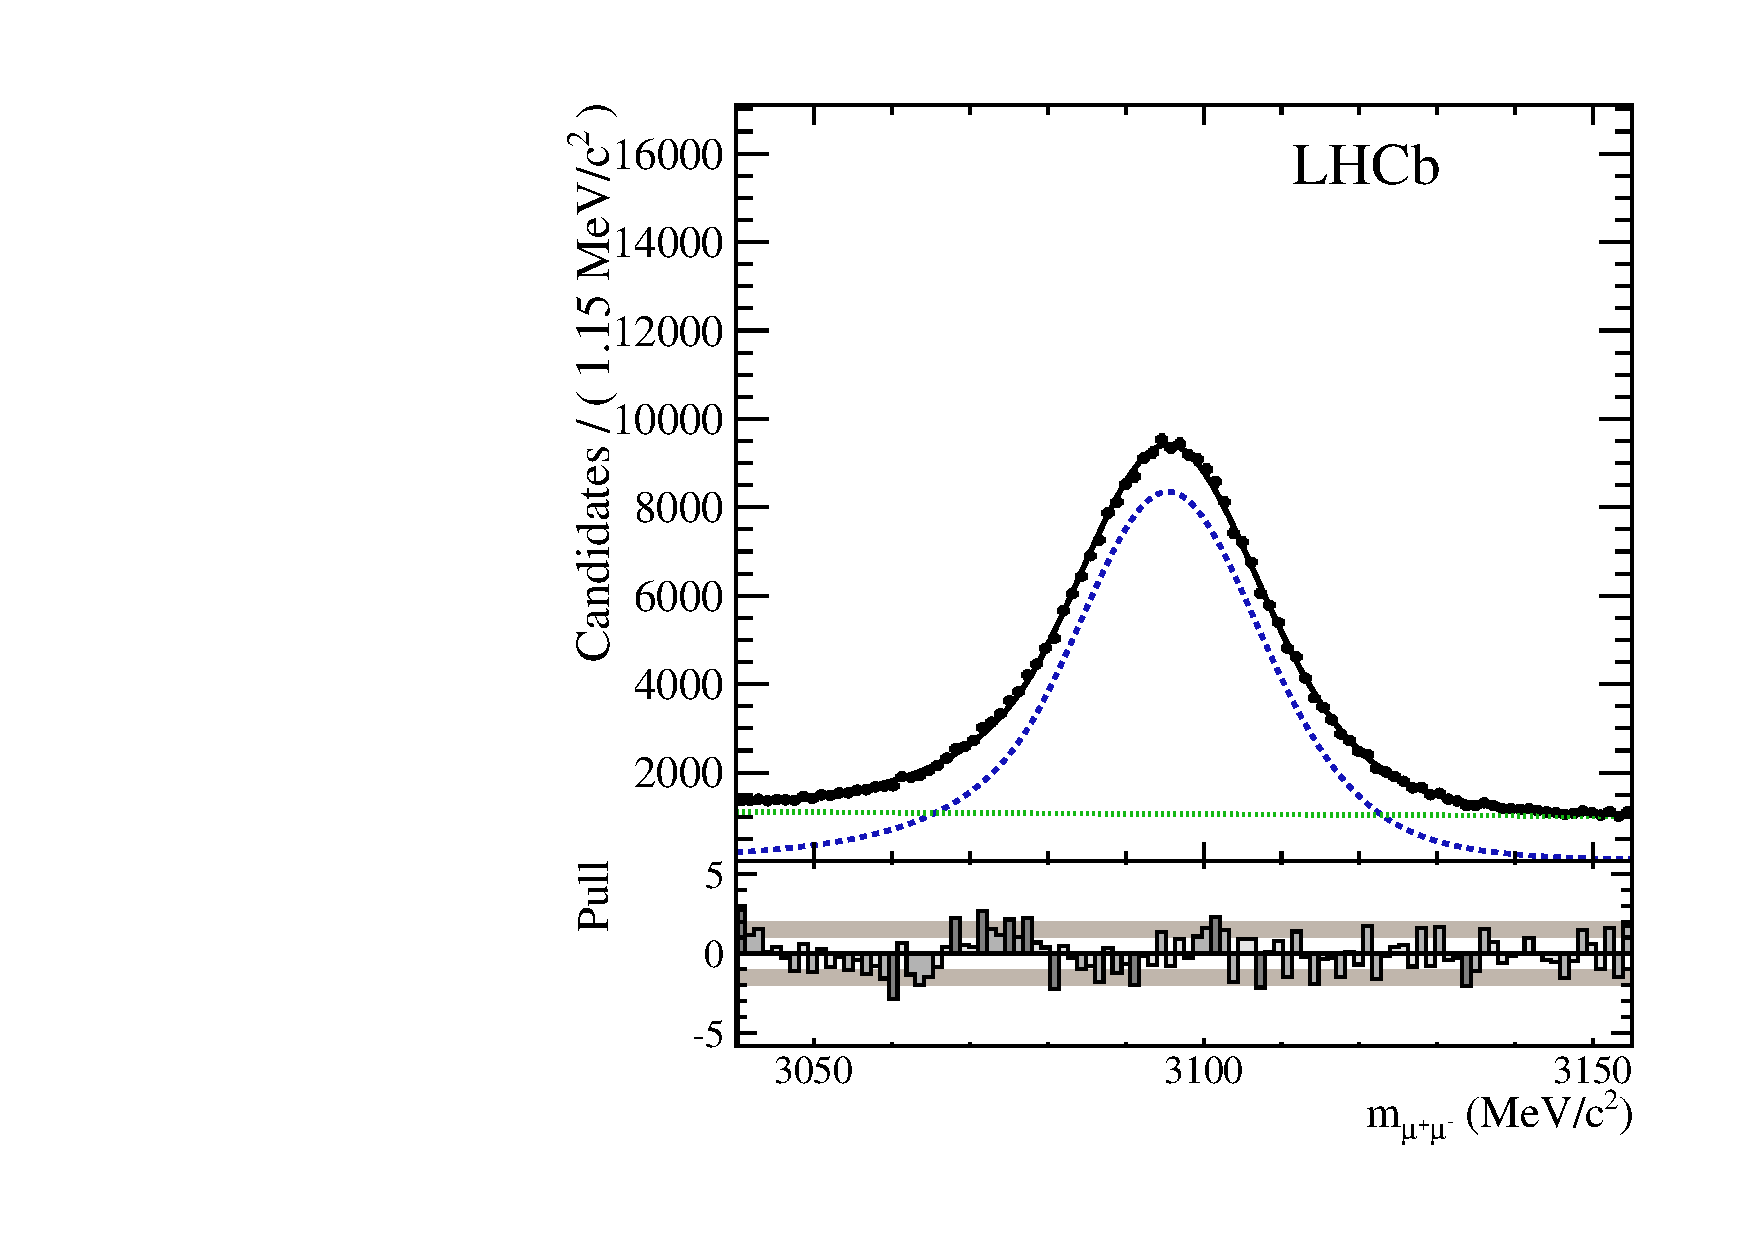
\includegraphics[width=0.49\textwidth]{private/content/measurement-of-sin2beta/figs/resolution_mass_jpsi_dd.pdf}
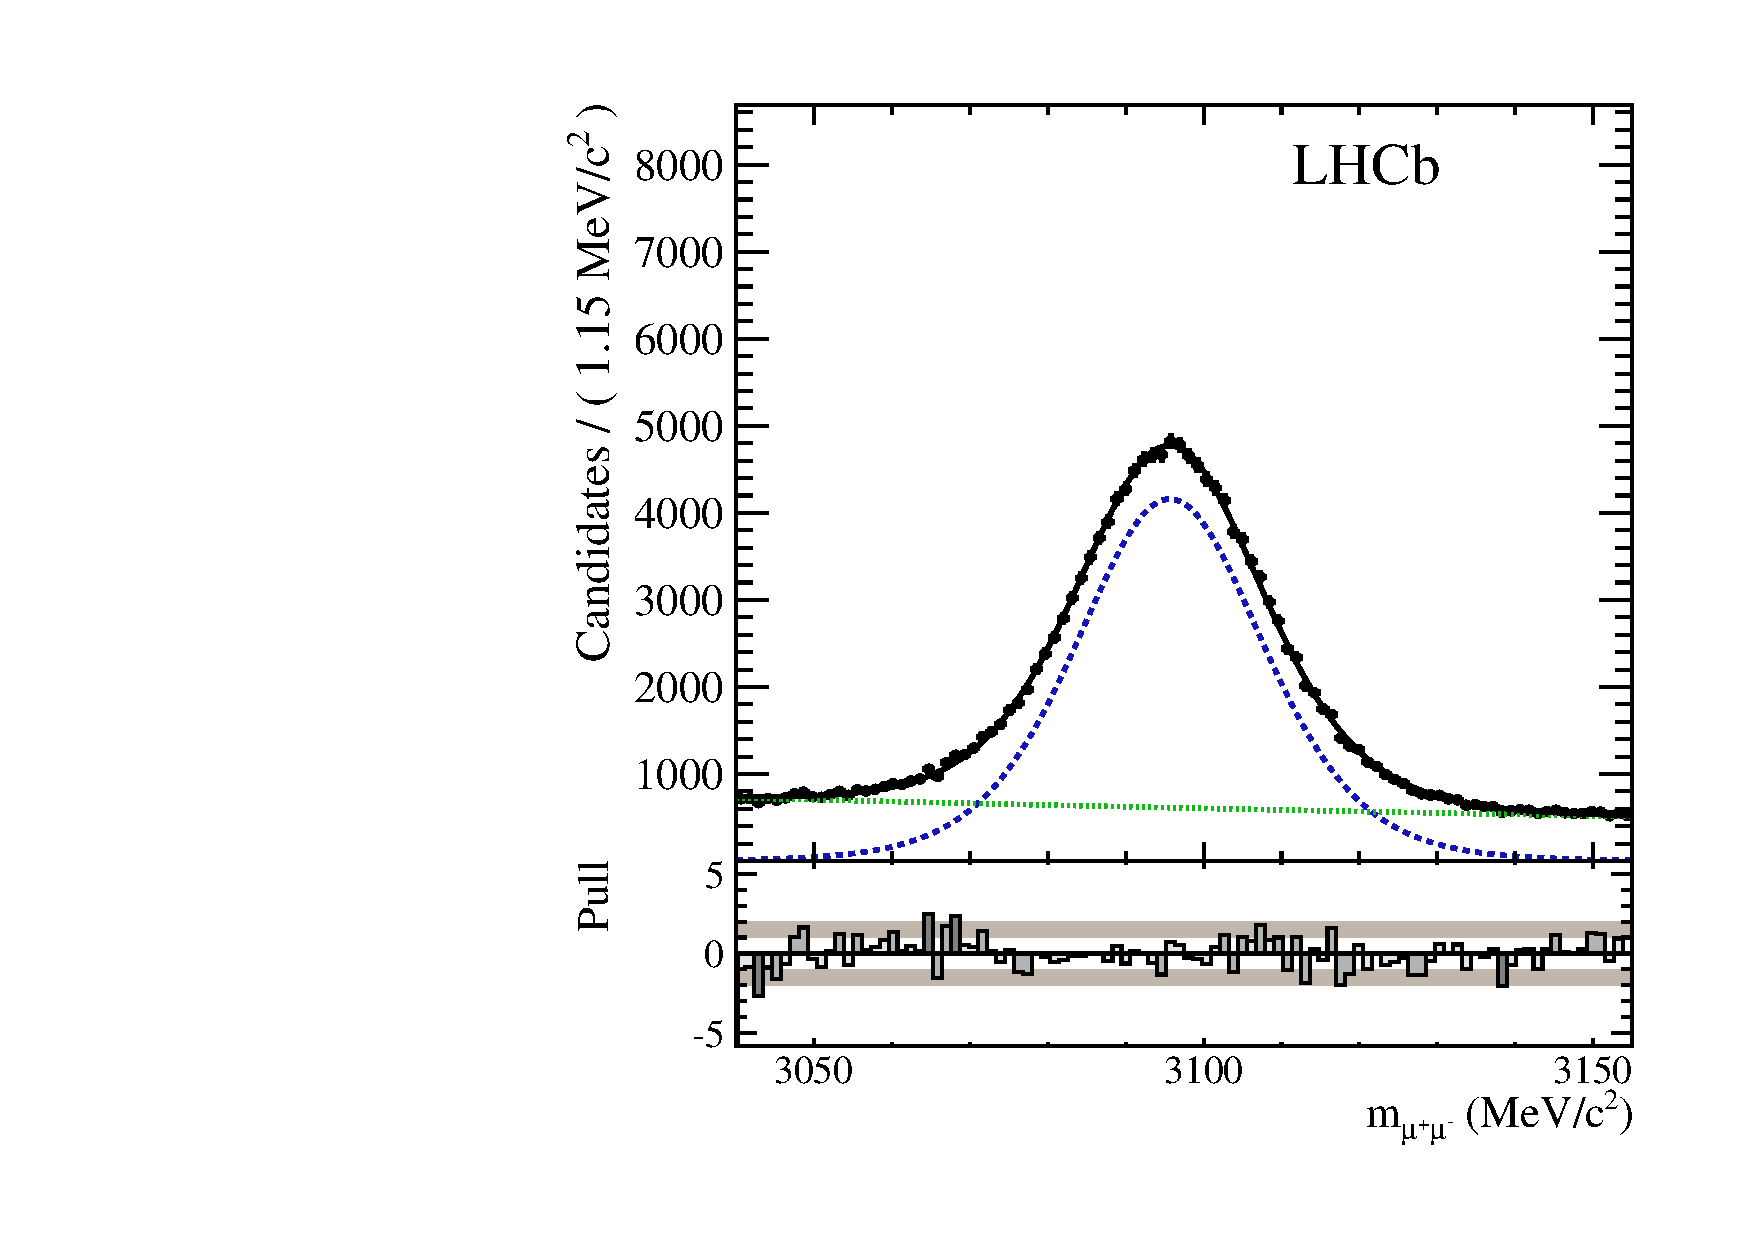
\includegraphics[width=0.49\textwidth]{private/content/measurement-of-sin2beta/figs/resolution_mass_jpsi_ll.pdf}
\caption{Invariant $\Jpsi$ candidate mass distribution in the (left) \catDD and
(right) \catLL subsample. Data are shown in black, the projection of the total
\acs{PDF} as solid black line, the signal component described by an Ipatia
\acs{PDF} as dashed blue line, and the exponential background component as
dotted green line.}
\label{fig:measurement_of_sin2beta:resolution_and_acceptance:resolution:jpsi_mass}
\end{figure}
%
Using a simultaneous fit in $\num{20}$ equally filled bins of the decay time
error prediction $\obsTimeError$ the width of the prompt peak in the decay time
distribution is fitted. The fit model consist of two Gaussian \acs{PDF} sharing
a common mean parameter to model the prompt peak and an additional decay \PDF as
parametrisation of the non-prompt component of true \BdToJpsiKS candidates. The
decay \PDF is convoluted with the same double-Gaussian \PDF used to model the
prompt peak. The two widths---one narrow and one wider---are then both employed
in the calibration.

For both widths a binned $\chisq$-fit of the $\num{20}$ per-bin parameter values
against the per-bin $\obsTimeError$ averages is performed. One linear and two
parabolic calibration models (with and without offset) are tested. For both
widths as well as for both the \catDD and \catLL candidates the linear model
$\sigma^\prime(\obsTimeError) = c_i + b_i \obsTimeError$ describes the data at
least equally well \wrt the other parametrisations, such that the simpler model
is chosen in case of comparable results.
\Cref{fig:measurement_of_sin2beta:resolution_and_acceptance:resolution:calibration} 
shows the calibration function for both track types and both Gaussian width
parameters.
%
\begin{figure}[h]
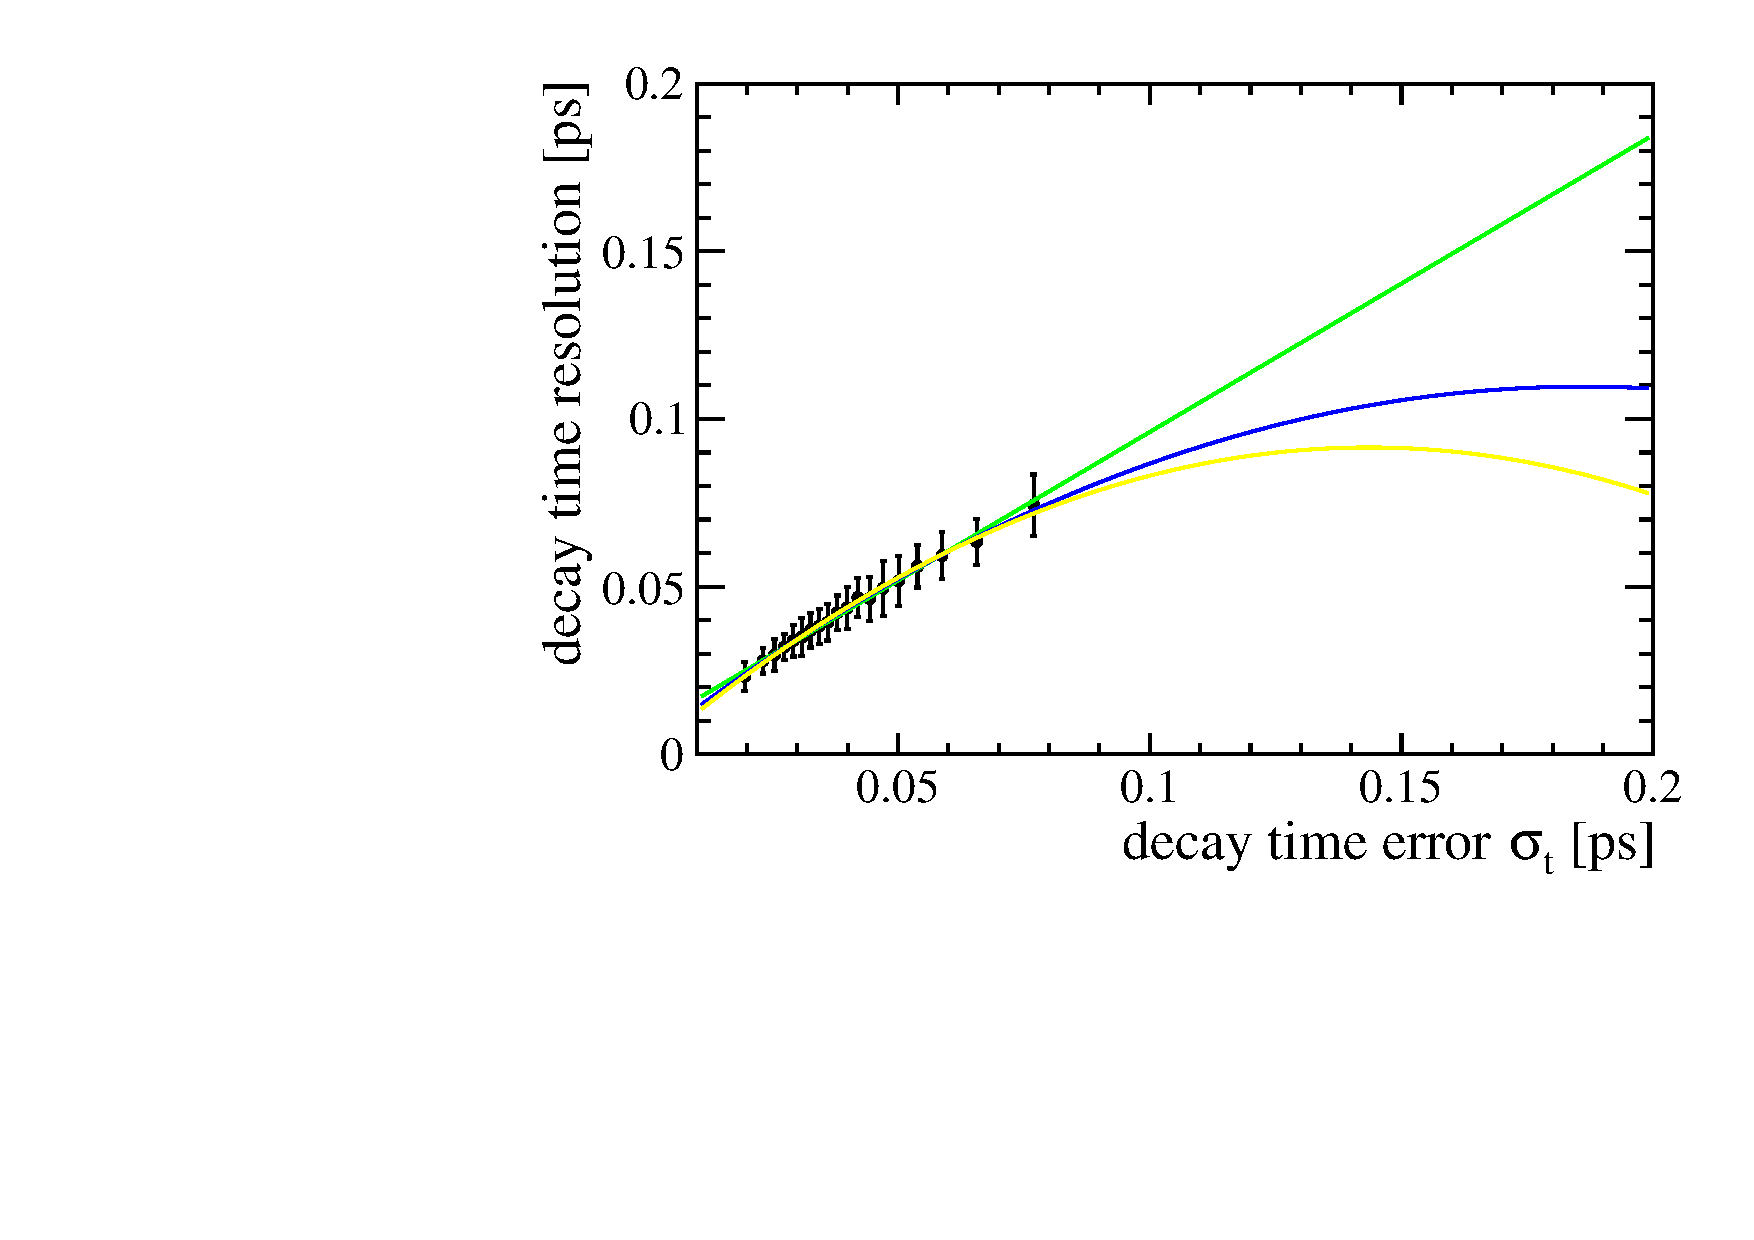
\includegraphics[width=0.49\textwidth]{private/content/measurement-of-sin2beta/figs/resolution_calibration_dd_narrow.pdf}
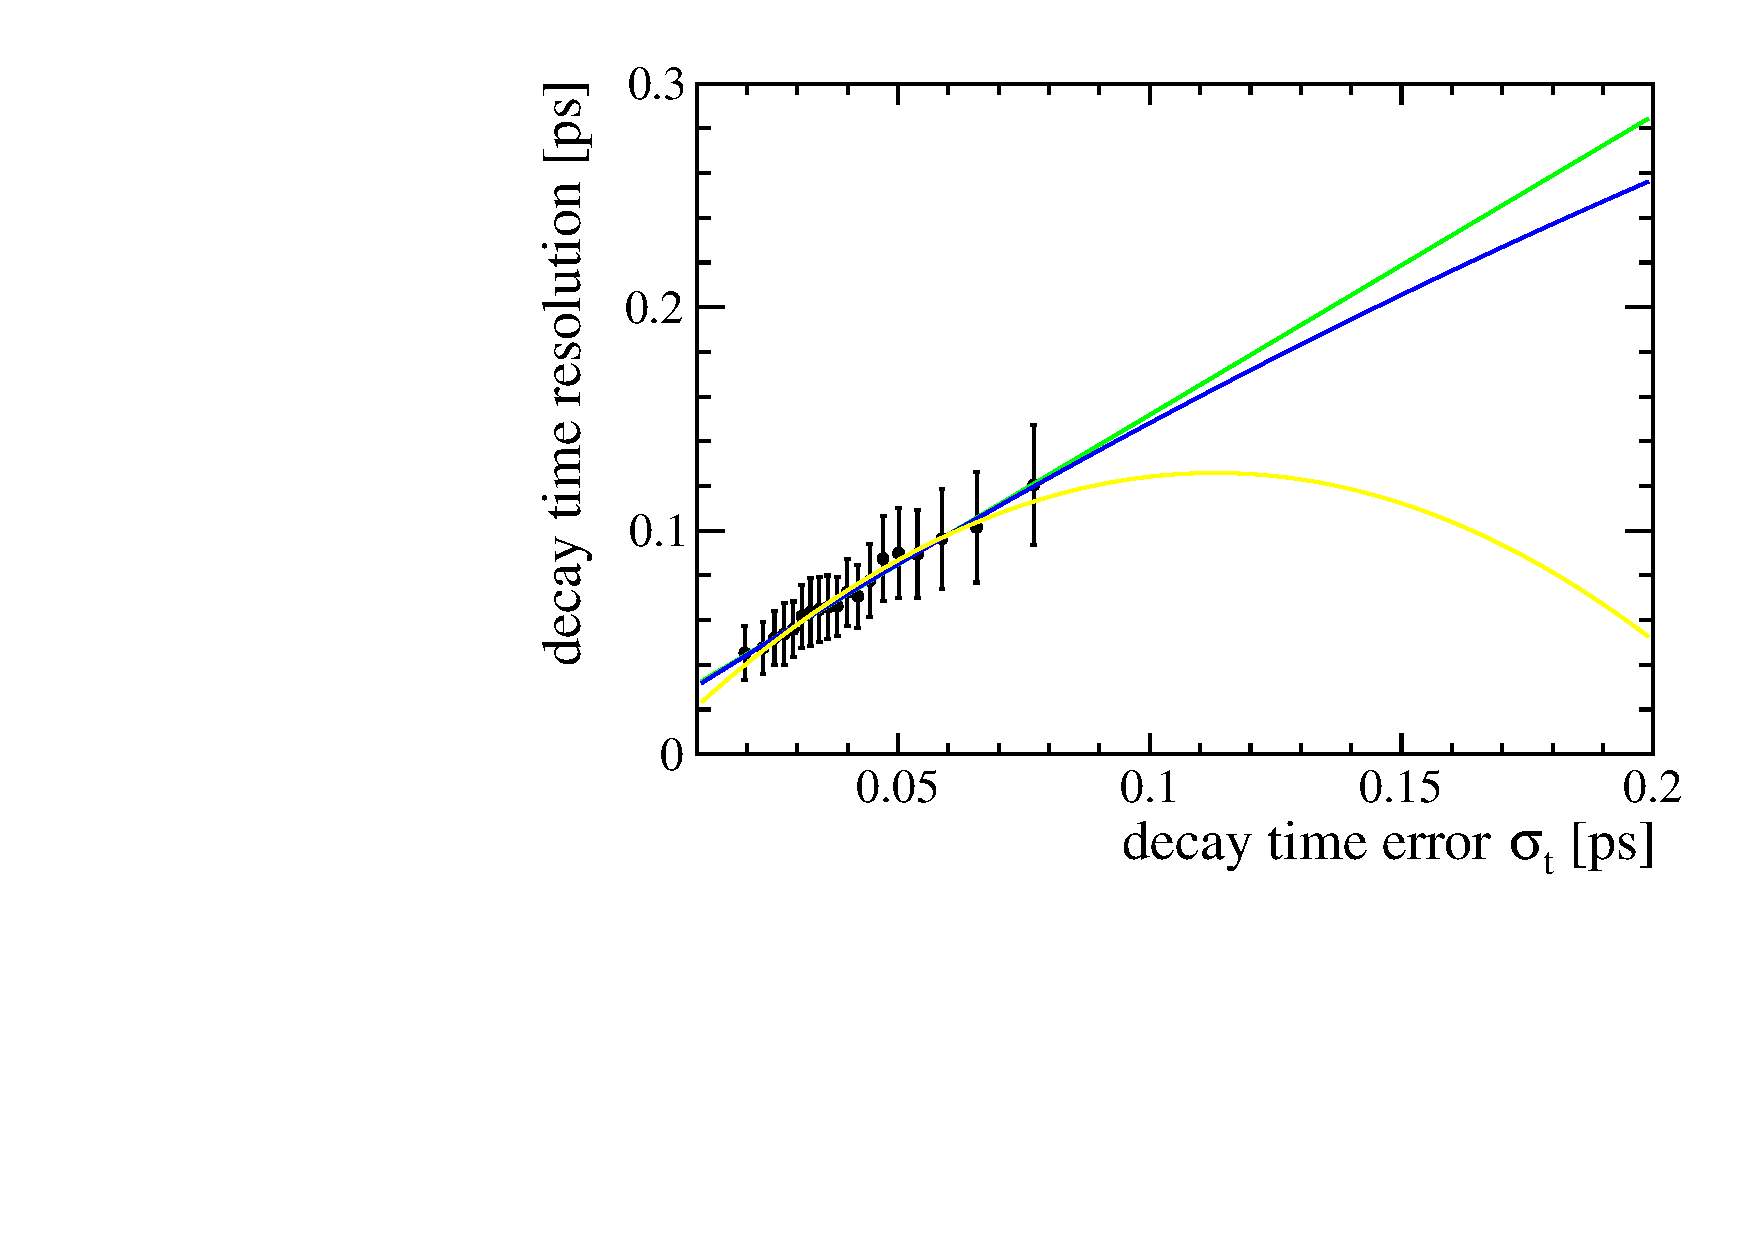
\includegraphics[width=0.49\textwidth]{private/content/measurement-of-sin2beta/figs/resolution_calibration_dd_wide.pdf}
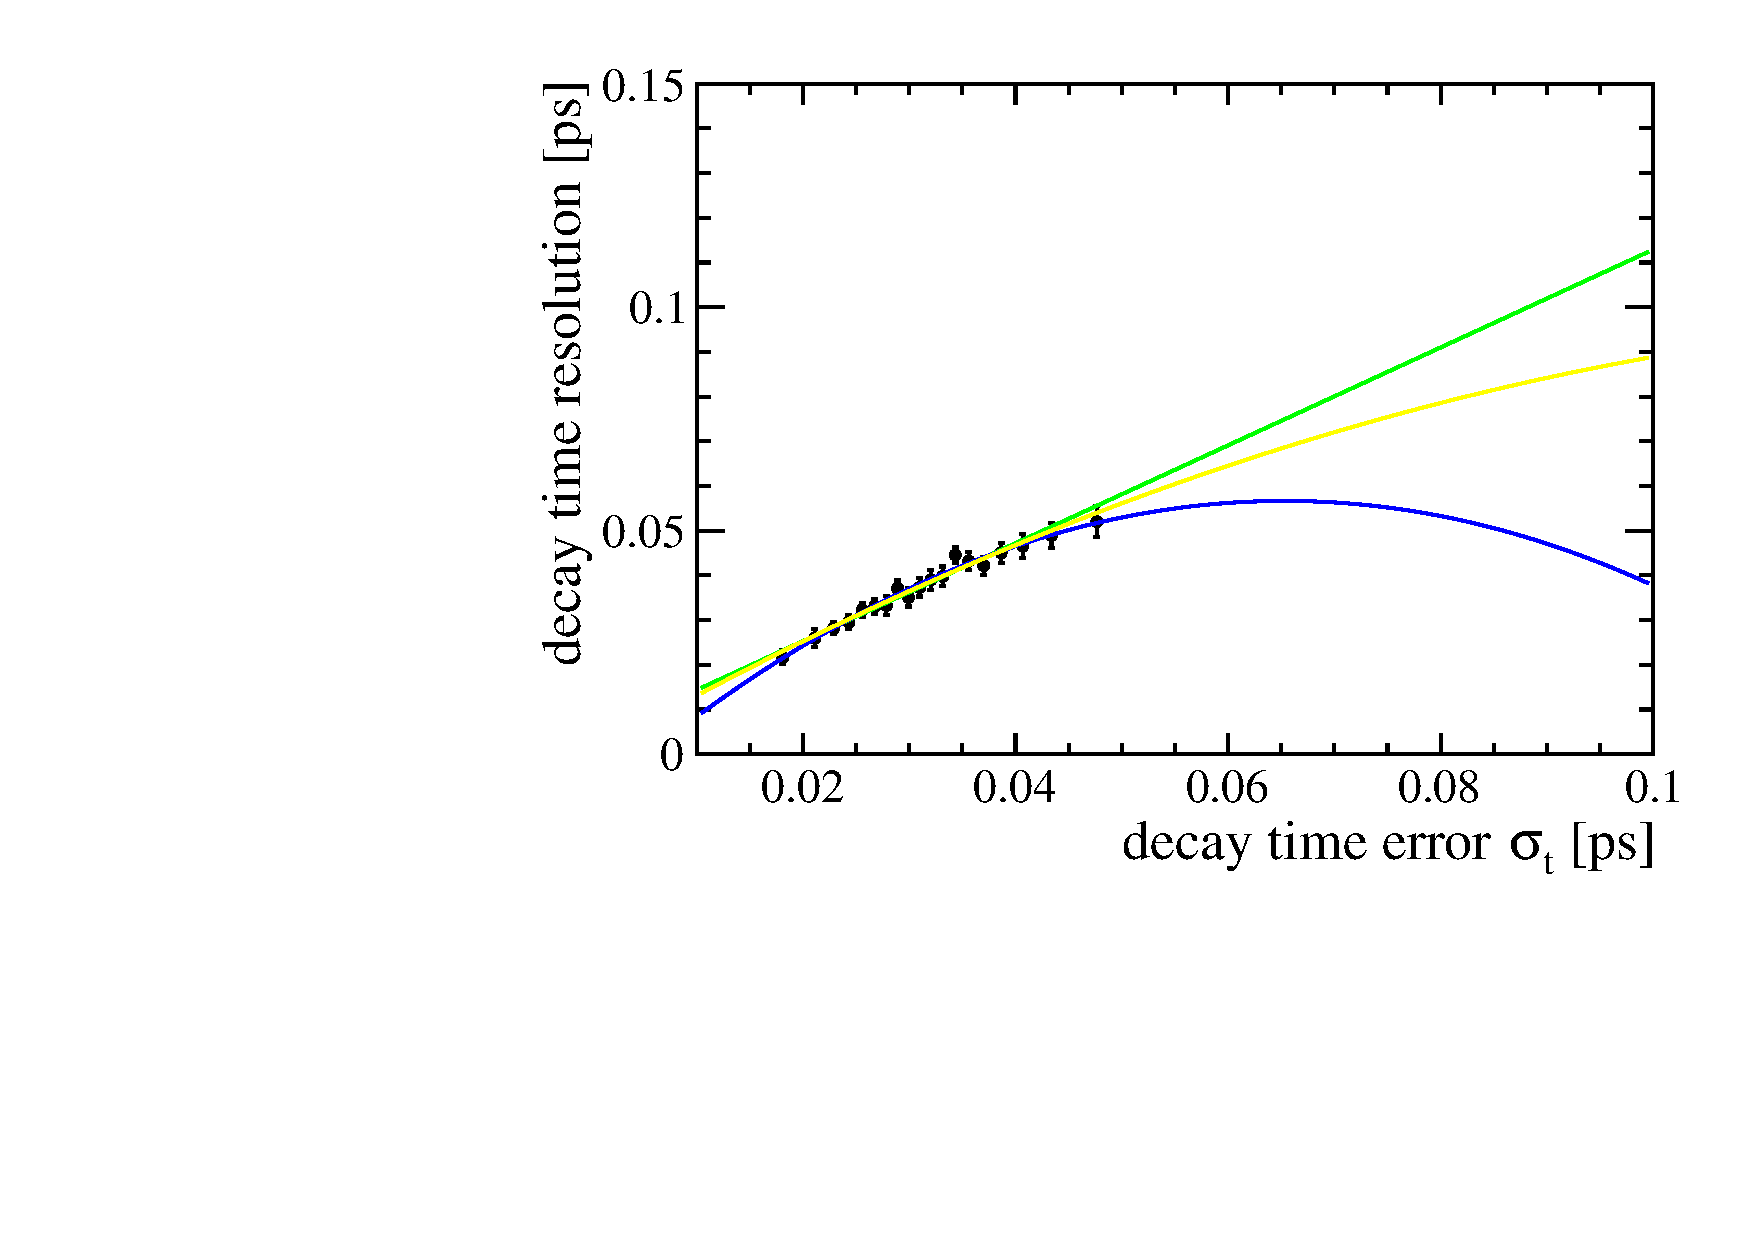
\includegraphics[width=0.49\textwidth]{private/content/measurement-of-sin2beta/figs/resolution_calibration_ll_narrow.pdf}
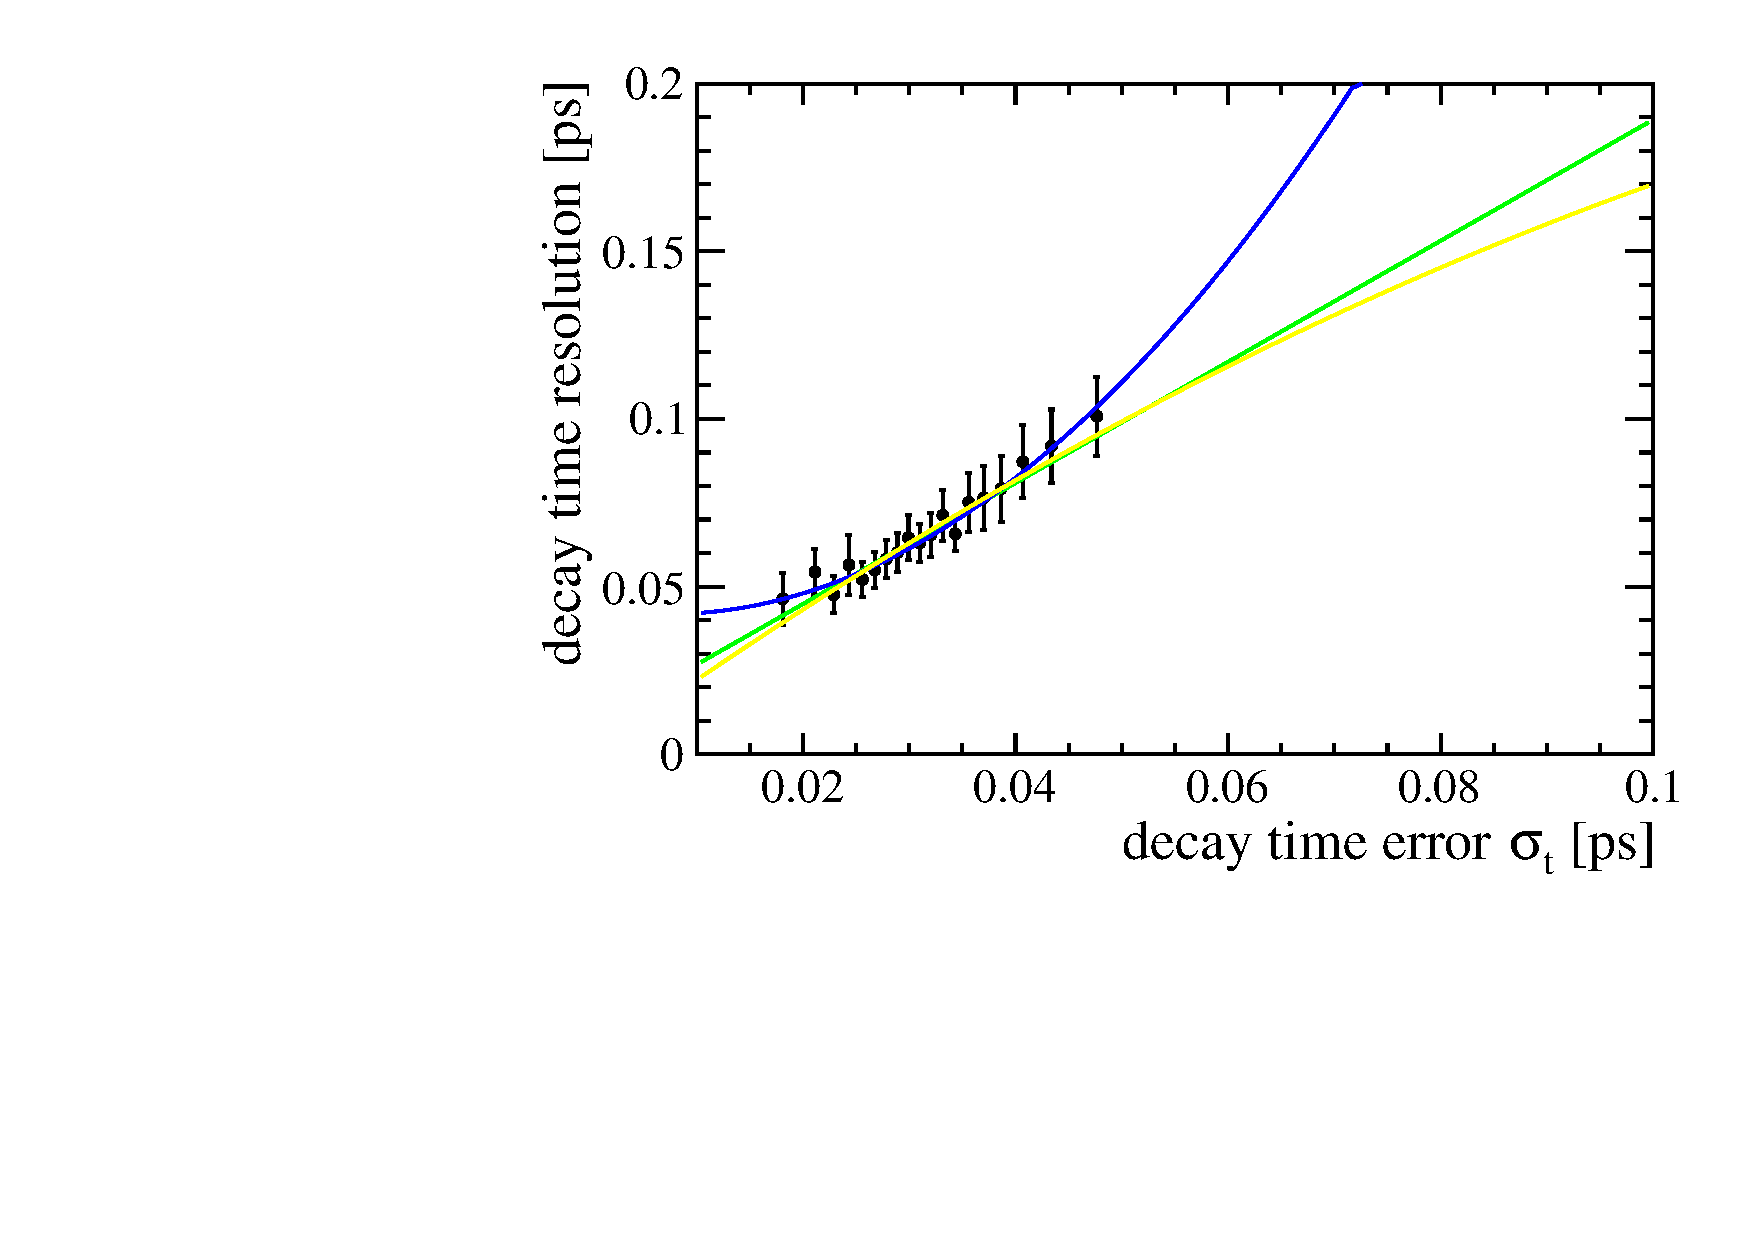
\includegraphics[width=0.49\textwidth]{private/content/measurement-of-sin2beta/figs/resolution_calibration_ll_wide.pdf}
\caption{Decay time error estimate calibration for (top) \catDD and (bottom)
\catLL candidates. Different calibration functions are fitted to the (left)
narrow and the (right) wide Gaussian width parameters. In green the linear
function $\sigma^\prime(\obsTimeError) = c_i + b_i \obsTimeError$ is shown, blue
and yellow describe the parabolic function with and without offset.}
\label{fig:measurement_of_sin2beta:resolution_and_acceptance:resolution:calibration}
\end{figure}
%
Results of the depicted fits are given in 
\cref{tab:app:measurement_of_sin2beta:resolution_and_acceptance:resolution:calibration:dd,tab:app:measurement_of_sin2beta:resolution_and_acceptance:resolution:calibration:ll}
in \cref{sec:app:measurement_of_sin2beta:resolution_and_acceptance:resolution}.

Using the determined calibration model, the nominal decay time resolution model
is developed. An unbinned maximum likelihood fit to the \Bd decay time is
performed on the same $\Jpsi$ signal \sweighted dataset as described before
using the resolution model
%
\begin{equation}\label{eq:measurement_of_sin2beta:resolution_and_acceptance:resolution}
\begin{split}
  \Resolution{}{}\left(\obsTime;\obsTimeError\right)
  &= \sum_{i=1}^{2}{g_i\,\cdot\,\frac{1}{\sqrt{2\pi}(c_i + b_i \cdot \obsTimeError)}\exp\left(-\frac{(\obsTime - \mu_t)^2}{2(c_i + b_i \cdot \obsTimeError)^2}\right)}\\
  &+ f_{\text{PV}} \frac{1}{\sqrt{2\pi} \sigma_{\text{PV}}} \exp\left(-\frac{(\obsTime - \mu_t)^2}{2 \sigma_{\text{PV}}^2}\right) \eqpd
\end{split}
\end{equation}
%
The first two Gaussian components describe the prompt peak resolution, the third
component models the distribution of candidates associated to the wrong \PV.
Different calibration parameters $c_i$ and $b_i$ are chosen for the width of the
narrow ($i=1$) and the wide ($i=2$) Gaussian \PDF. The fractions $g_i$ add up to
unity together with the fraction $f_\text{\acs*{PV}}$ of candidates associated
to the wrong \PV. The offset $\mu_{\obsTime}$ of the Gaussian central value is
shared between all three Gaussian \acp{PDF}. Finally,
$\sigma_{\text{\acs*{PV}}}$ describes the width of the wrong \PV component.
\Cref{tab:measurement_of_sin2beta:resolution_and_acceptance:resolution:calibration:results} 
lists the results that are used from now on in the decay time resolution model.
How the choice of the calibration model influences the measurement is tested
using a \ToyMC study described in
\cref{sec:measurement_of_sin2beta:systematics:systematics:resolution}
%
\begin{table}[!htb]
\centering
\caption{Results of the fit of the parameters described in the decay time
resolution model.}
\label{tab:measurement_of_sin2beta:resolution_and_acceptance:resolution:calibration:results}
  \begin{tabular}{llr@{$\,\pm\,$}lr@{$\,\pm\,$}l}
    \toprule
    \multicolumn{2}{c}{Parameter}       &   \multicolumn{2}{c}{\catDD sample}   &   \multicolumn{2}{c}{\catLL sample}\\
    \midrule
    $\mu_t$             &   (\si{\ps})  &   -0.00291    &   0.00026                 &   -0.00169    &   0.00026     \\
    $b_{1}$             &               &   0.88        &   0.09                    &   1.04        &   0.14      \\
    $c_{1}$             &   (\si{\ps})  &   0.0077      &   0.0028                  &   0.0045      &   0.0028      \\
    $b_{2}$             &               &   1.33        &   0.33                    &   1.8         &   0.4      \\
    $c_{2}$             &   (\si{\ps})  &   0.019       &   0.008                   &   0.007       &   0.005         \\
    $g_{2}$             &               &   0.251       &   0.020                   &   0.24        &   0.023      \\
    $\sigma_\text{PV}$  &   (\si{\ps})  &   1.6         &   0.7                     &   1.40        &   0.14    \\
    $f_\text{PV}$       &               &   0.048       &   0.004                   &   0.0488      &   0.0024  \\
    \midrule
    $\tau_1$            &   (\si{\ps})  &   0.7         &   0.5                     &   0.29        &   0.06     \\
    $\tau_2$            &   (\si{\ps})  &   2.1         &   1.3                     &   1.82        &   0.12     \\
    $f_1$               &               &   0.08        &   0.10                    &   0.046       &   0.006     \\
    $f_2$               &               &   0.08        &   0.11                    &   0.079       &   0.009     \\
    \bottomrule
  \end{tabular}
\end{table}

% ------------------------------------------------------------------------------
\subsection{Decay time acceptance}
\label{sec:measurement_of_sin2beta:resolution_and_acceptance:acceptance}

Acceptance effects that alter the distribution of the decay time might result
from selection requirements or inefficiencies in the event reconstruction.
\Cref{sec:measurement_of_sin2beta:resolution_and_acceptance:acceptance:lower}
summarises acceptance effects stemming from lifetime biasing selection cuts from
the trigger requirements
(\cf \cref{sec:measurement_of_sin2beta:data_preparation:trigger}). Reconstruction
inefficiencies mainly caused by the \VELO track reconstruction algorithms (\cf
\cref{sec:lhcb_experiment:tracking}) are outlined in
\cref{sec:measurement_of_sin2beta:resolution_and_acceptance:acceptance:upper}.

% ..............................................................................
\subsubsection{Trigger induced decay time acceptance}
\label{sec:measurement_of_sin2beta:resolution_and_acceptance:acceptance:lower}

The biased trigger lines (\cf
\cref{sec:measurement_of_sin2beta:data_preparation:trigger}) and the stripping
cut on the reconstructed decay time of the $\Bd$ candidates result in a non-flat
decay time acceptance.

In order to correctly describe these effects, the data sample is split into two
disjoint categories of candidates that show a substantially different behaviour
regarding their decay time acceptance. All candidates passing the \emph{almost
unbiased} (\textbf{\catAU}) trigger requirements show nearly no decay time
acceptance effects, in contrast to the sample of candidates passing the
\emph{exclusively biased} (\textbf{\catEB}) trigger requirements. The addressed
requirements are:
%
\begin{description}
  \item[\catAU] \TriggerReqAU
  \item[\catEB] \TriggerReqEB
\end{description}
%
To construct the acceptance in terms of ratios, a sample of candidates that pass
a set of unbiased trigger requirements is needed:
%
\begin{description}
  \item[Unbiased] \TriggerReqUB
\end{description}
%
The acceptance of the \catAU subsample can be computed using the overlap of events
which pass both the \HLTTwoDiMuonDetachedJpsi and the
\HLTTwoDiMuonJpsi line. Both lines are using the same trigger cuts except for
an additional cut on the flight distance significance (see
\cref{tab:measurement_of_sin2beta:data_preparation:trigger:hlt2:cuts}) in the
case of the biased lines. The acceptance can then be written as a time-dependent
efficiency $\varepsilon_\text{\catAU}$, with
%
\begin{equation}
  \begin{split}
    \varepsilon_\text{\catAU} &= \frac{\VerbAU \VerbAnd \HLTTwoDiMuonJpsi}{\VerbUB}\\
                              &= \frac{\TriggerReqAUEnumerator}{\TriggerReqUB}.
  \end{split}
\end{equation} 
%
For the \catEB subsample, there is no corresponding reference sample available,
so strictly speaking only a relative efficiency can be computed. Nonetheless,
the ratio of the \catEB subsample and the unbiased subsample can be computed as
$\varepsilon_\text{\catEB}$.
%
\begin{equation}
  \begin{split}
    \varepsilon_\text{\catEB} &= \frac{\VerbEB}{\VerbUB}\\
                              &= \frac{\TriggerReqEB}{\TriggerReqUB}
  \end{split}
\end{equation}
%
In other words $\varepsilon_\text{\catAU}$ quantifies the efficiency due to the
\HLTTwoDiMuonDetachedJpsi requirement, whereas $\varepsilon_\text{\catEB}$
effectively quantifies the relative efficiency due to the \HLTOneTrackMuon
requirement.

\subsubsection*{Methodology}
% \label{sec:propertime:methodology}

The data set for studying the trigger acceptance effects consists of all events
that are selected by the \StrippingDetached stripping line and pass the
offline selection. As the tagged and untagged candidates are expected to behave
equally concerning the studied effect all available candidates are used.
On the remaining multiple candidates, a random candidate selection is applied.
All candidates are selected by one of the following trigger lines:
\HLTOneDiMuonHighMass, \HLTOneTrackMuon, \HLTTwoDiMuonJpsi, or
\HLTTwoDiMuonDetachedJpsi.

The efficiencies are time-dependent and, since the focus lies on the acceptance
of the signal component's decay time distribution, have to be determined through
a fit. To do so, a simultaneous fit for the signal yield is performed in ten
bins of decay time. The bin boundaries are chosen in a way that each bin
contains the same number of events (before splitting the data into the different
fit categories). The fit is also performed simultaneously in categories of track
type, tagger, and both trigger sets given by the numerators of
$\varepsilon_\text{\catAU}$ and $\varepsilon_\text{\catEB}$. The yields for the
different tagger and track type categories are summarized (including error
propagation). Then the efficiency per time bin is calculated. For
$\varepsilon_{\catAU}$ a binomial error is estimated, while a Gaussian error
propagation is used for $\varepsilon_{\catEB}$.

In the mass fit, the signal peak is described by a double Gaussian with a shared
mean, while a single exponential is used to describe the combinatorial
background. 
\Cref{fig:measurement_of_sin2beta:resolution_and_acceptance:acceptance:lower:mass_fits} 
shows both mass distributions and fit projections for the biased and unbiased
sample, respectively. In both plots the sum over all categories is displayed.
%
\begin{figure}
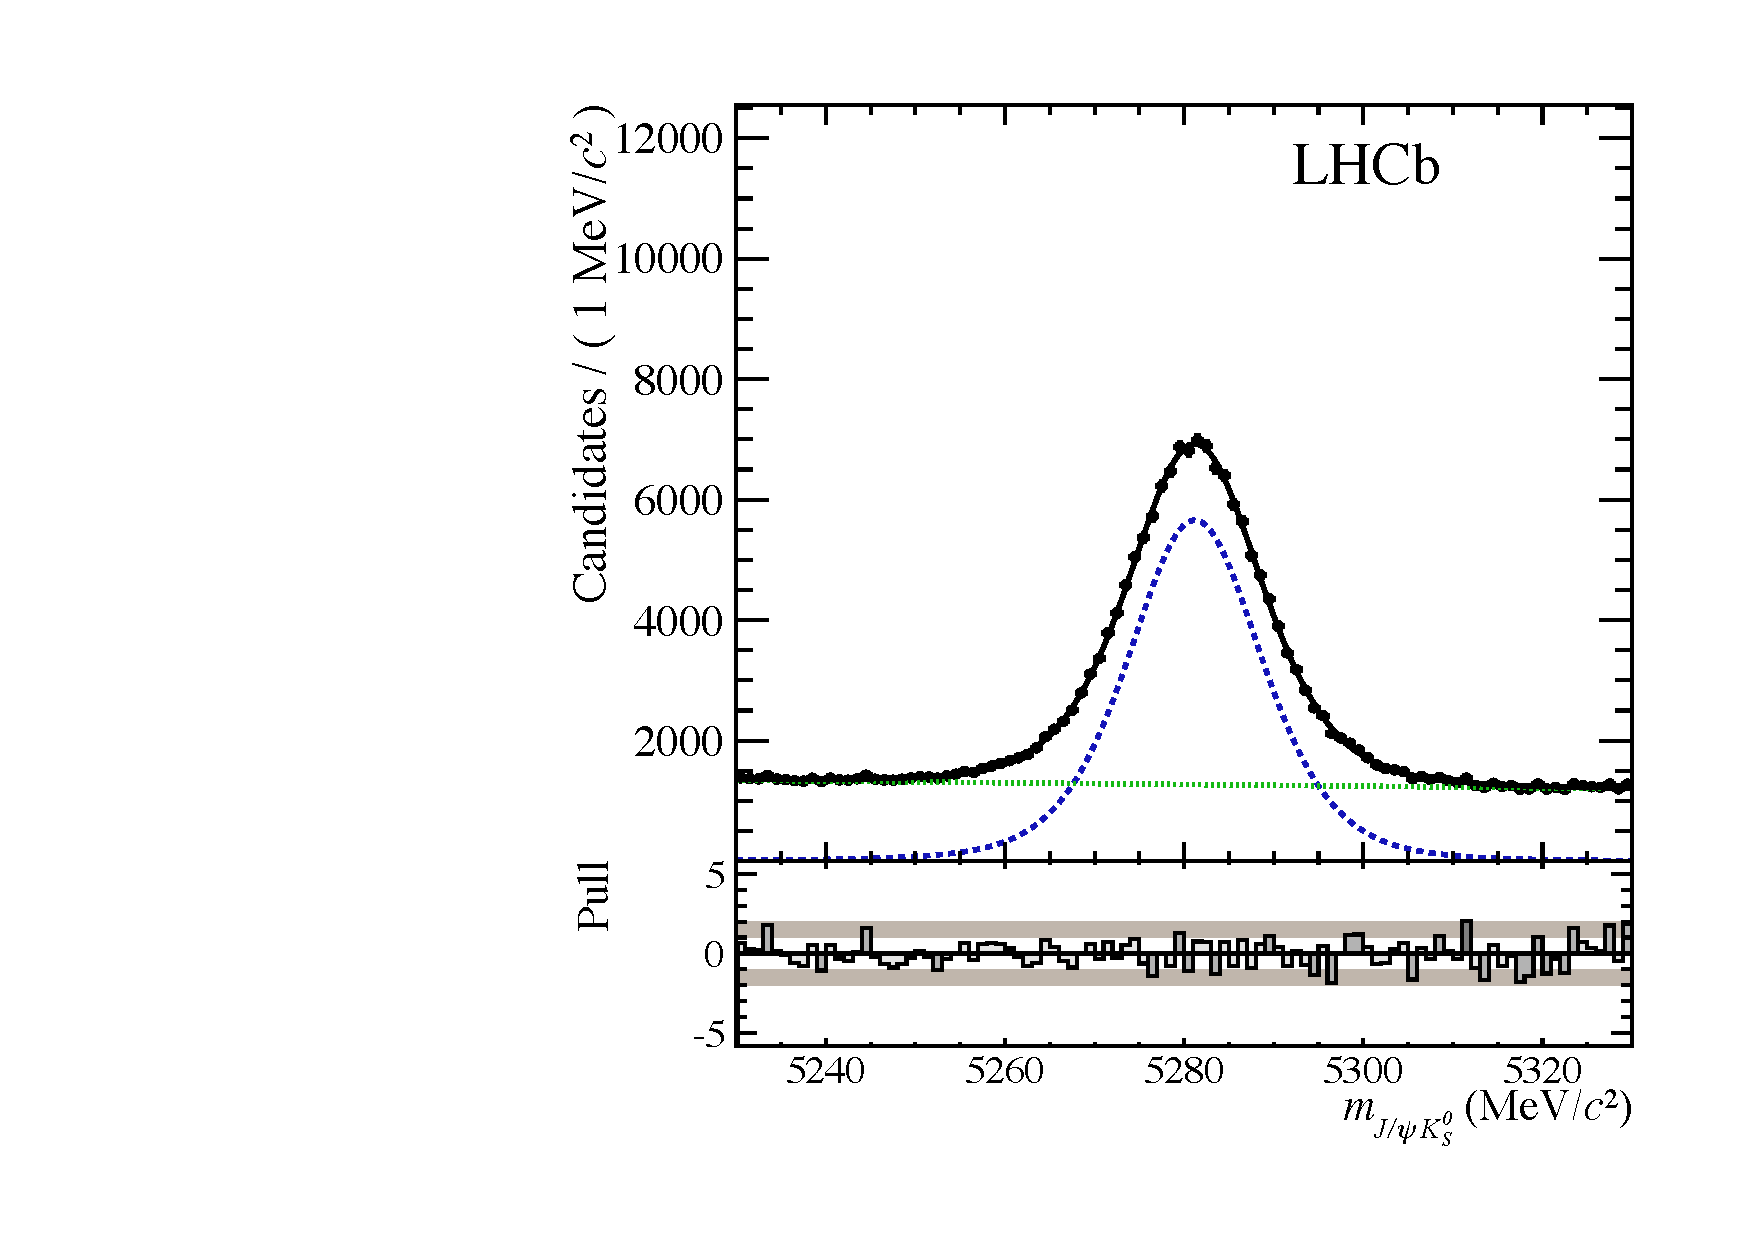
\includegraphics[width=0.49\textwidth]{private/content/measurement-of-sin2beta/figs/mass_trigger_efficiency_biased.pdf}
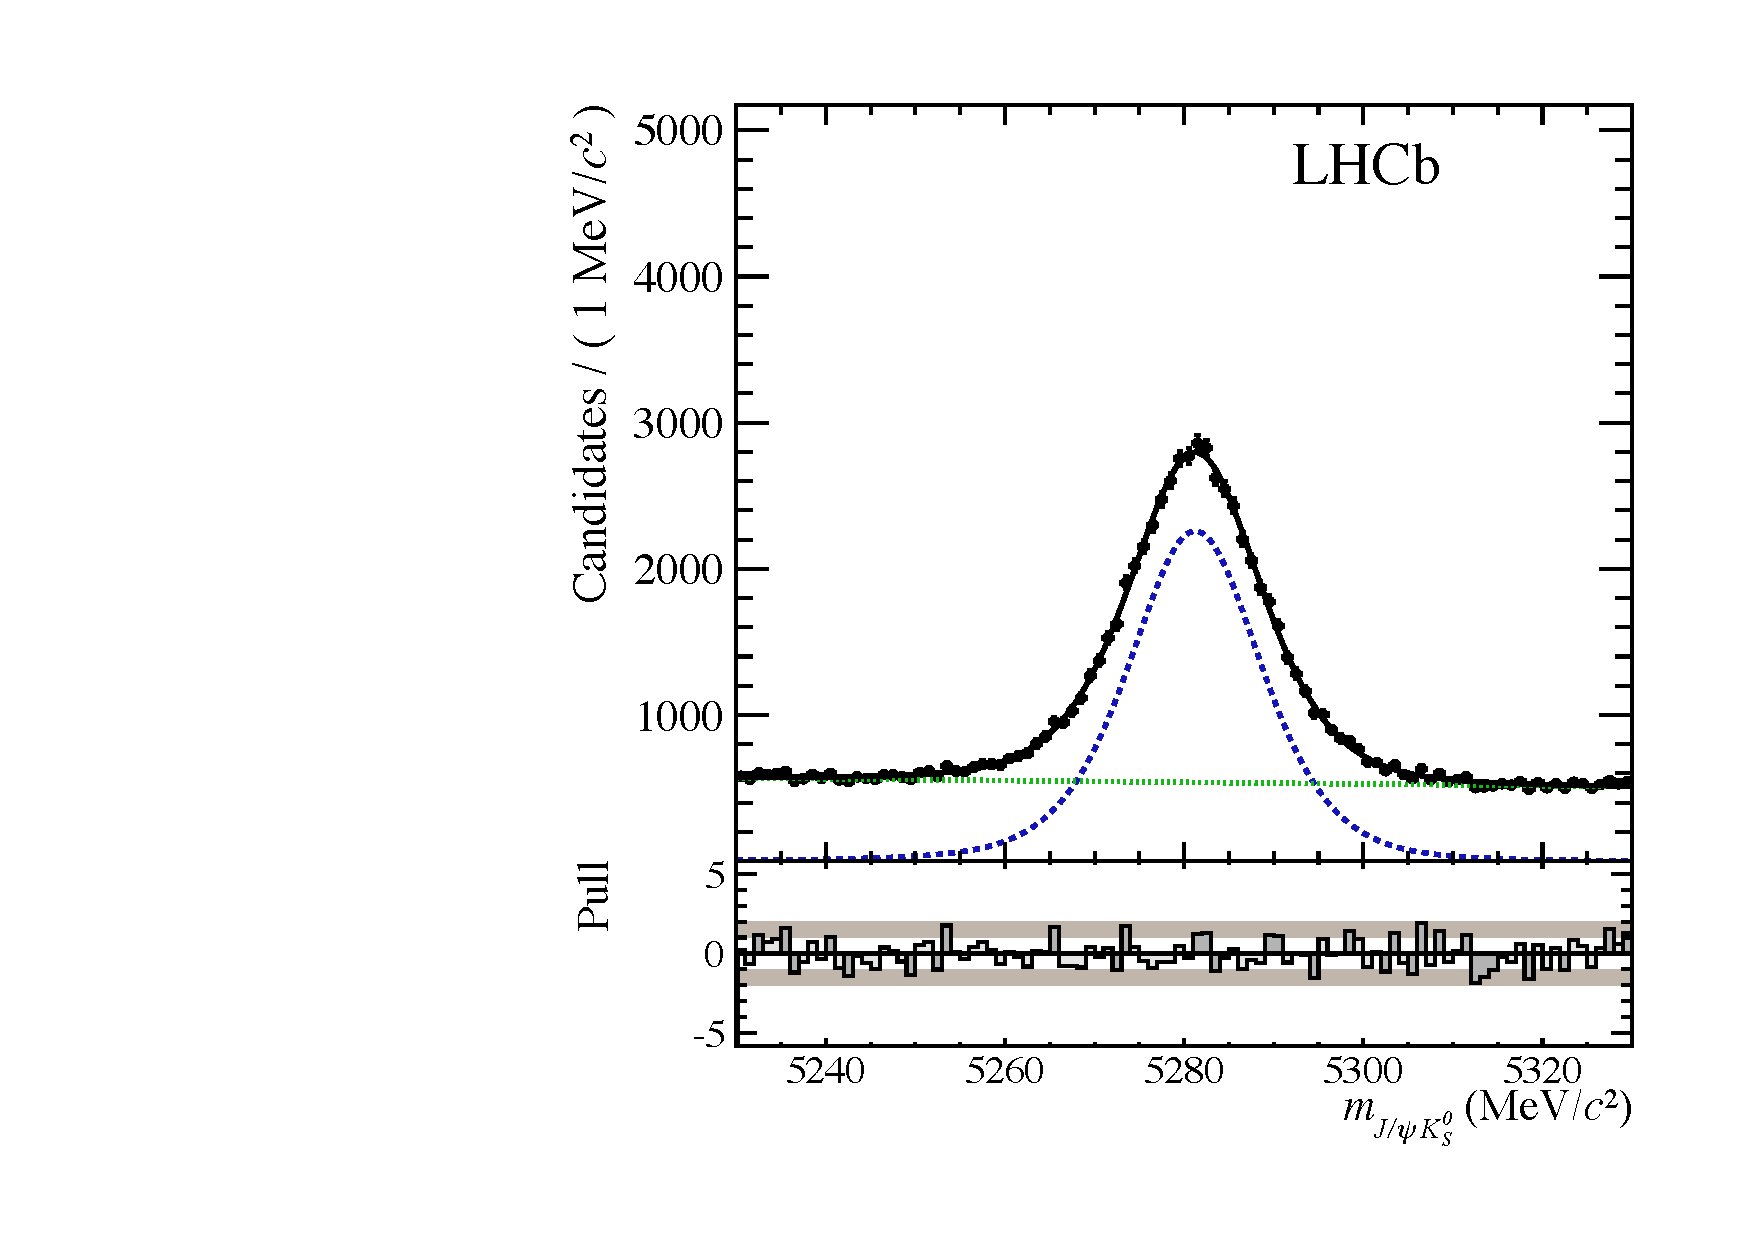
\includegraphics[width=0.49\textwidth]{private/content/measurement-of-sin2beta/figs/mass_trigger_efficiency_unbiased.pdf}
\label{fig:measurement_of_sin2beta:resolution_and_acceptance:acceptance:lower:mass_fits}
\caption{Mass distribution and fit projection summarised over all categories for
the (left) biased (\catAU and \catEB) and the (right) unbiased sample.}
\end{figure}
%
\Cref{fig:measurement_of_sin2beta:resolution_and_acceptance:acceptance:lower:splines} 
shows the acceptance histograms for the \catAU and the \catEB sample. In the
nominal fit we use cubic splines\addref{Cubic splines} instead of the histograms
themselves. Each bin centre is used as a knot for the splines. The bin contents
determine the shape of the splines. However, the bin contents aren't fixed but
constrained with a Gaussian function where the width is given by the uncertainty
on the bin content. As there is no information about the acceptance at the decay
time limits, the efficiency is assumed to be flat between the lower decay time
limit at \SI{0.3}{\ps} and the first bin centre/knot and the last bin
centre/knot and the upper decay time limit at
\SI{18.3}{\ps}, respectively.
%
\begin{figure}
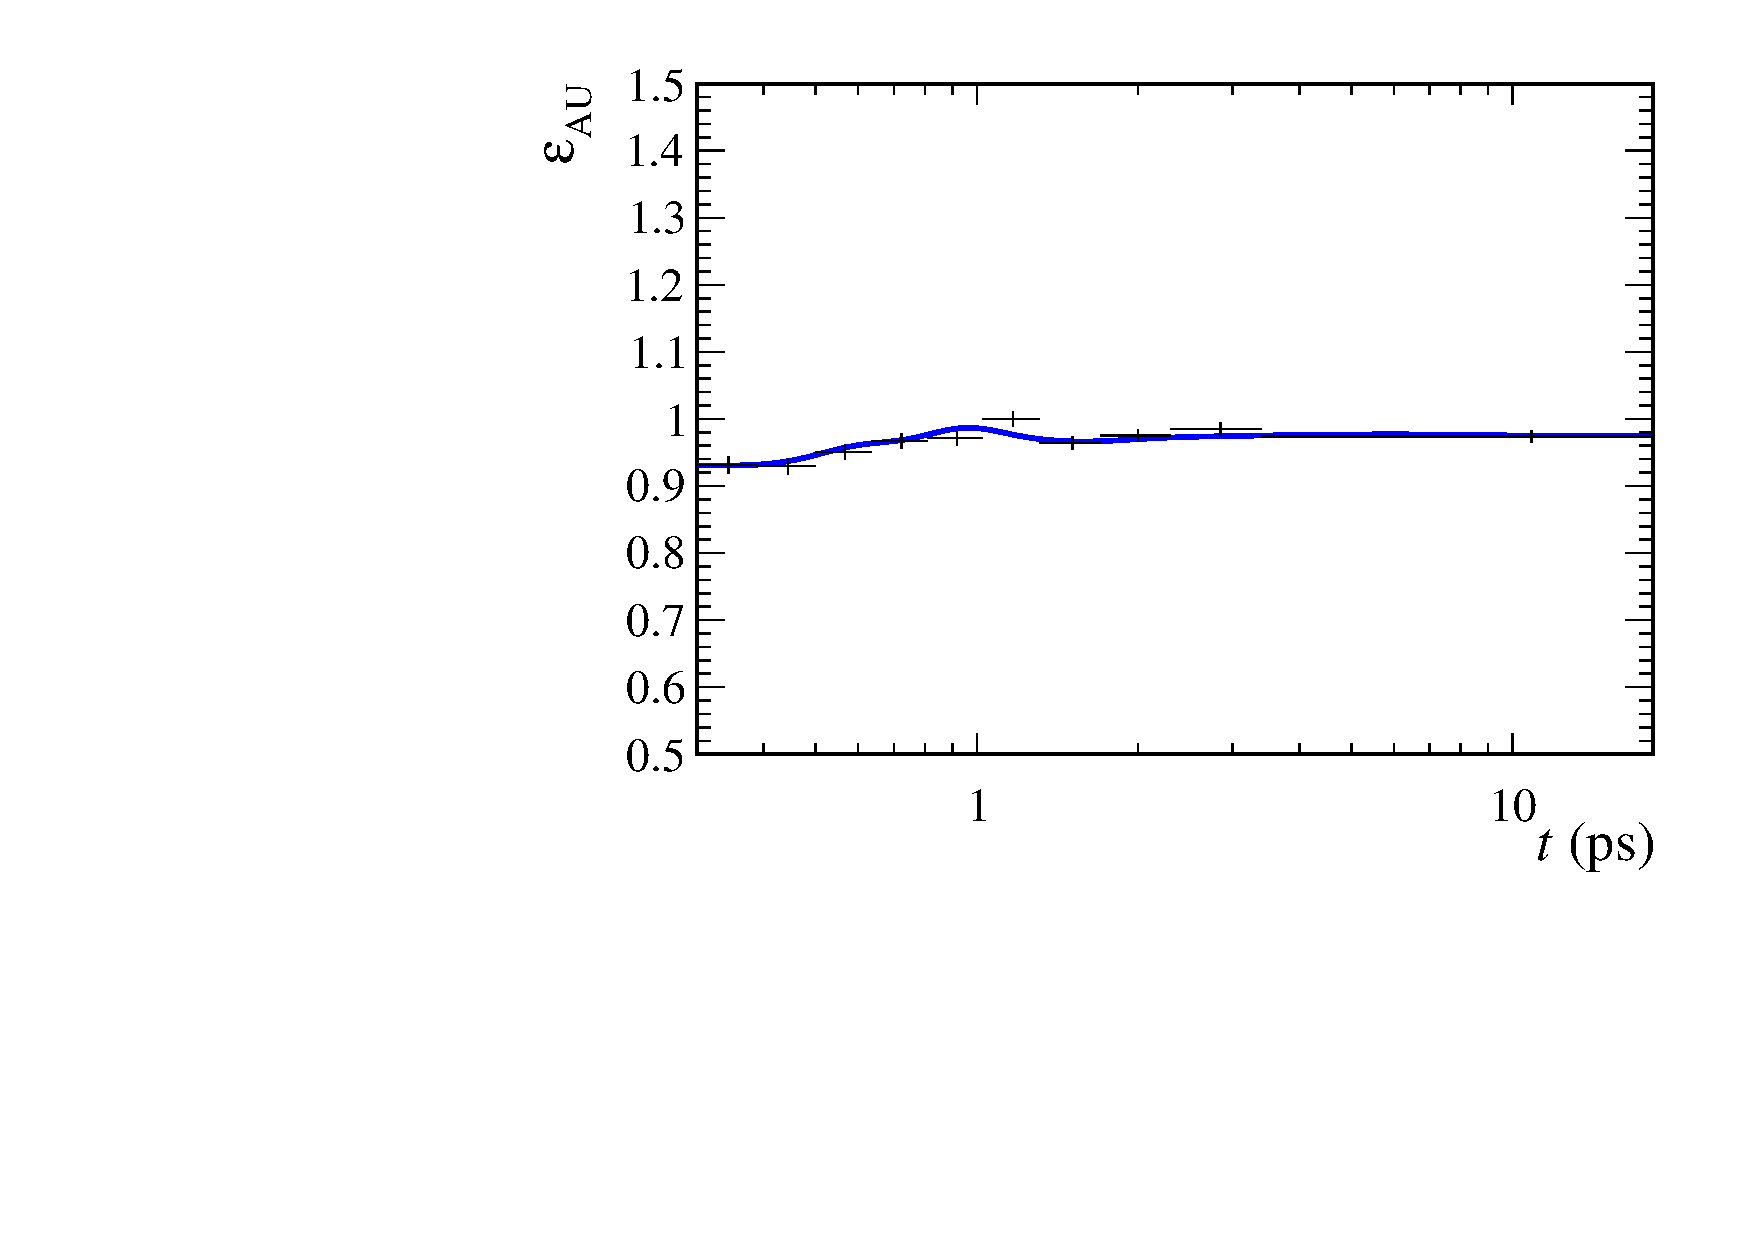
\includegraphics[width=0.49\textwidth]{private/content/measurement-of-sin2beta/figs/trigger_acceptance_spline_AU.pdf}
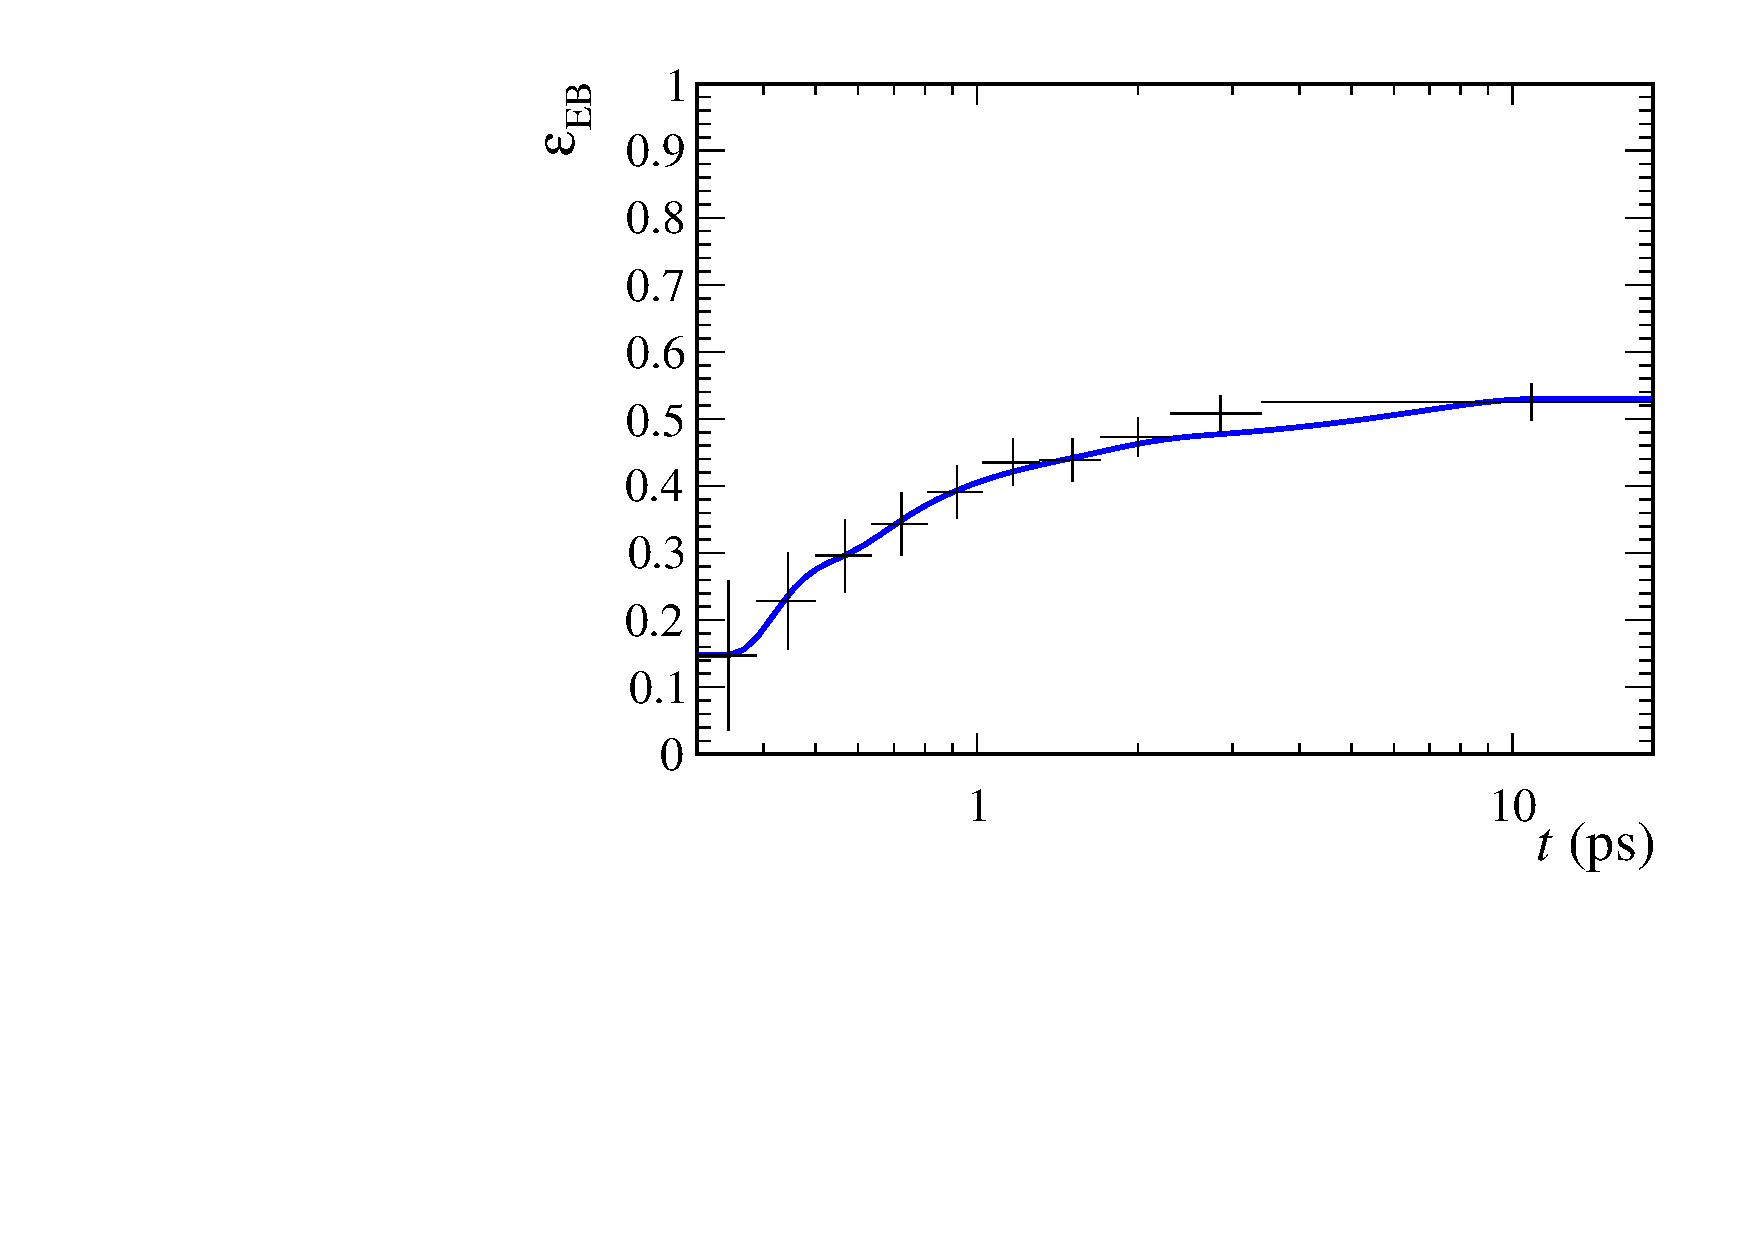
\includegraphics[width=0.49\textwidth]{private/content/measurement-of-sin2beta/figs/trigger_acceptance_spline_EB.pdf}
\label{fig:measurement_of_sin2beta:resolution_and_acceptance:acceptance:lower:splines}
\caption{Histograms of the trigger acceptance for the (left) almost unbiased and
the (right) exclusively biased sample. The blue curve shows the fitted
acceptance using cubic splines.}
\end{figure}

% ..............................................................................
\subsubsection{Upper decay time acceptance}
\label{sec:measurement_of_sin2beta:resolution_and_acceptance:acceptance:upper}

Due to the \VELO reconstruction inefficiency\todo{Be more precise, FastVelo
algorithm} and other reconstruction and selection effects, a second decay time
acceptance is observed for events with larger decay times. To account for
this a correction factor $\beta_\tau$ is included into the fit model
by implementing the modified lifetime
%
\begin{equation}
  \widetilde{\tau} = \frac{\tau}{1 + \beta_\tau \tau} ,
\end{equation}
%
which expands to\info{Stop expansion after linear term?}
%
\begin{equation}\label{eq:measurement_of_sin2beta:resolution_and_acceptance:acceptance:upper:linear}
\begin{split}
  \Prob{}{}\left(t\right) &= \exponential{-\frac{t}{\tau}\left(1+\beta_{\tau}\tau\right)} \\
                          &= \exponential{-\frac{t}{\tau}-\beta_{\tau}t} = \exponential{-\frac{t}{\tau}} \exponential{-\beta_{\tau}t} \\
                          &= \exponential{-\frac{t}{\tau}}\left(1-\beta_{\tau} t+\frac{\beta_{\tau}^2 t^2}{2}+\order{\left((\beta_{\tau} t)^3\right)}\right).
\end{split}
\end{equation}
%
The value of $\beta_\tau$ is determined using a fit to simulated data while
fixing the lifetime $\tau$ to its generation value. Based on the
\BdToJpsiKS signal \MC data set, only candidates passing the
\StrippingPrescaled stripping line and the unbiased trigger lines
\HLTOneDiMuonHighMass and \HLTTwoDiMuonJpsi are chosen to avoid any
additional lifetime bias for events with short decay times. Only candidates
being matched on \MC as true signal events are considered. The nominal offline
selection is applied and from the remaining multiple (\acs{PV},\Bd) candidate pairs,
one is chosen randomly. To avoid wrong-\acs{PV} associations of the reconstructed
\BdToJpsiKS candidate the true \MC decay time is used in the fit. To reduce the
statistical uncertainties and as no deviations of the decay time distributions
are expected all untagged events are included. The number of remaining \MC
candidates available for this study is roughly \num{60000}. Due to differences
in the reconstruction efficiency the $\beta_\tau$ factor is determined
separately for \catOO/\catOT and \catDD/\catLL events
(\cref{tab:measurement_of_sin2beta:resolution_and_acceptance:acceptance:upper}\info{write a proper sentence}).
%
\begin{table}
  \centering
  \caption{Decay time correction factor $\beta_\tau$ in \si{\per\pico\second}.}
  \begin{tabular}{ccc}
    \toprule
     & 2011 & 2012 \\
    \midrule
    \catDD & $0.0036\pm0.0029$ & $0.0084\pm0.0032$ \\
    \catLL & $0.018\pm0.004$   & $0.035\pm0.005$ \\
    \bottomrule
  \end{tabular}
  \label{tab:measurement_of_sin2beta:resolution_and_acceptance:acceptance:upper}
\end{table}

\subsubsection*{Influence of higher order effects}
\todo{Leave out this possibility?}
To check the influence of higher order terms, a quadratic correction function is
tested where the second order term has an own degree of freedom given by
$\gamma_\tau$,
%
\begin{equation}\label{eq:measurement_of_sin2beta:resolution_and_acceptance:acceptance:upper:quadratic}
  \Prob{}{}\left(t\right) = \exponential{-\frac{t}{\tau}}\left(1-\beta_\tau t+ \gamma_\tau t^2\right).
\end{equation}
%
Again the parameters $\beta_\tau$ and $\gamma_\tau$ are fitted while fixing the
lifetime $\tau$. In \cref{tab:measurement_of_sin2beta:resolution_and_acceptance:acceptance:upper:quadratic} 
the results are listed for \catOO/\catOT and \catDD/\catLL events. To visualise
the effect, the per-bin ratio of the decay time distributions of signal \MC
events to events generated from \ToyMC is calculated and shown in
\cref{fig:measurement_of_sin2beta:resolution_and_acceptance:acceptance:upper}.
The \ToyMC decay time distribution follows an exponential function with the same
lifetime as used in the generation of the signal \MC. As the uncertainties on
$\beta_\tau$ and $\gamma_\tau$ are large and the parameters are strongly
correlated ($\rho>\SI{90}{\percent}$), the linear model is selected. A possible
bias due to this choice is investigated in
\cref{sec:measurement_of_sin2beta:systematics:systematics:acceptance}.
%
\begin{table}
  \centering
  \caption{Decay time correction factors $\beta_\tau$ (in \si{\per\pico\second})
  and $\gamma_\tau$ (in \si{\per\square\pico\second}).}
  \label{tab:measurement_of_sin2beta:resolution_and_acceptance:acceptance:upper:quadratic}
  \begin{tabular}{ccccc}
    \toprule
     & \multicolumn{2}{c}{2011} & \multicolumn{2}{c}{2012} \\
     & $\beta_\tau$ & $\gamma_\tau$ & $\beta_\tau$ & $\gamma_\tau$ \\
    \midrule
    \catDD & $-0.016\pm0.007$ & $-0.0030\pm0.0008$ & $-0.001\pm0.007$         & $-0.0014\pm0.0009$\\ 
    \catLL & $-0.001\pm0.009$ & $-0.0028\pm0.0012$ & $\phantom{+}0.01\pm0.06$ & $-0.0027\pm0.0008$\\ 
    \bottomrule
  \end{tabular}
\end{table}
%
\begin{figure}
  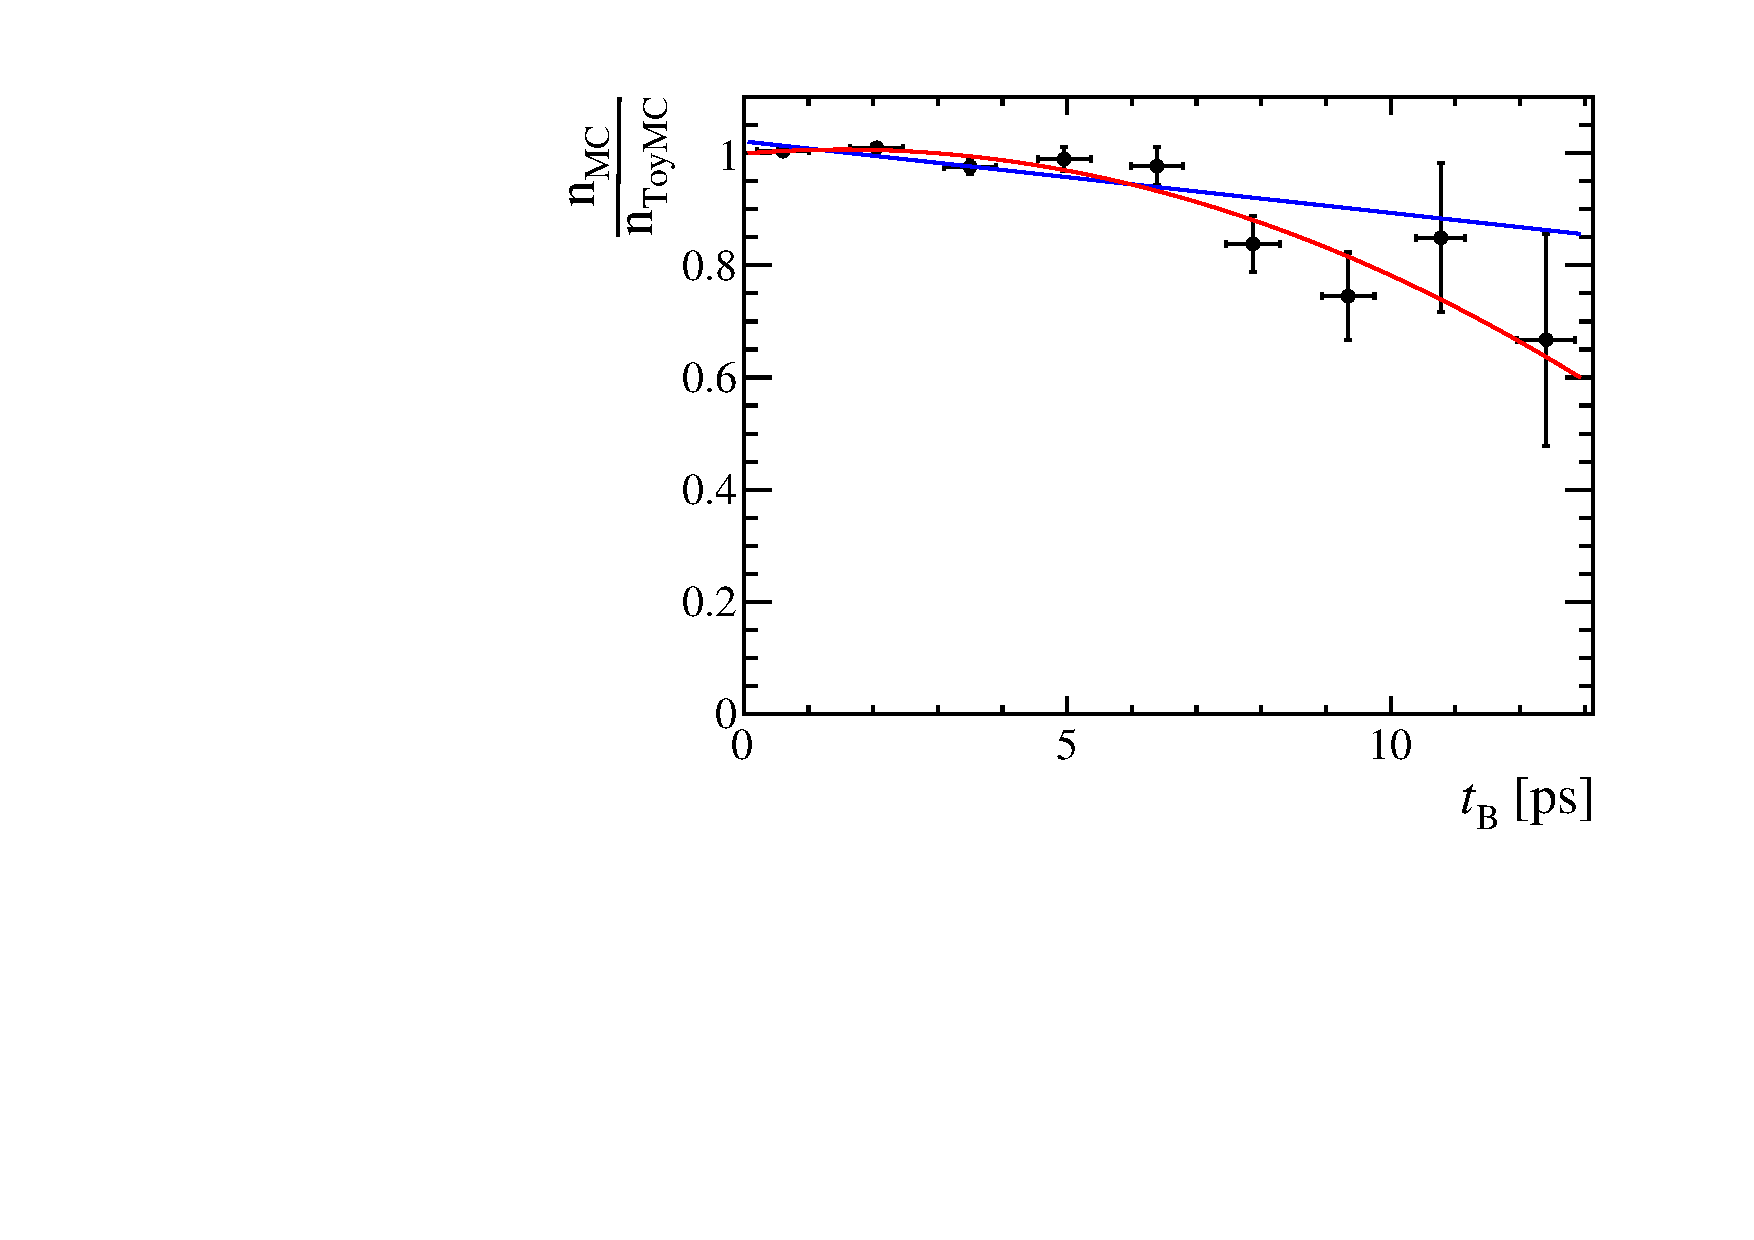
\includegraphics[width=0.49\textwidth]{private/content/measurement-of-sin2beta/figs/velo_acceptance_11_DD.pdf}\hfill
  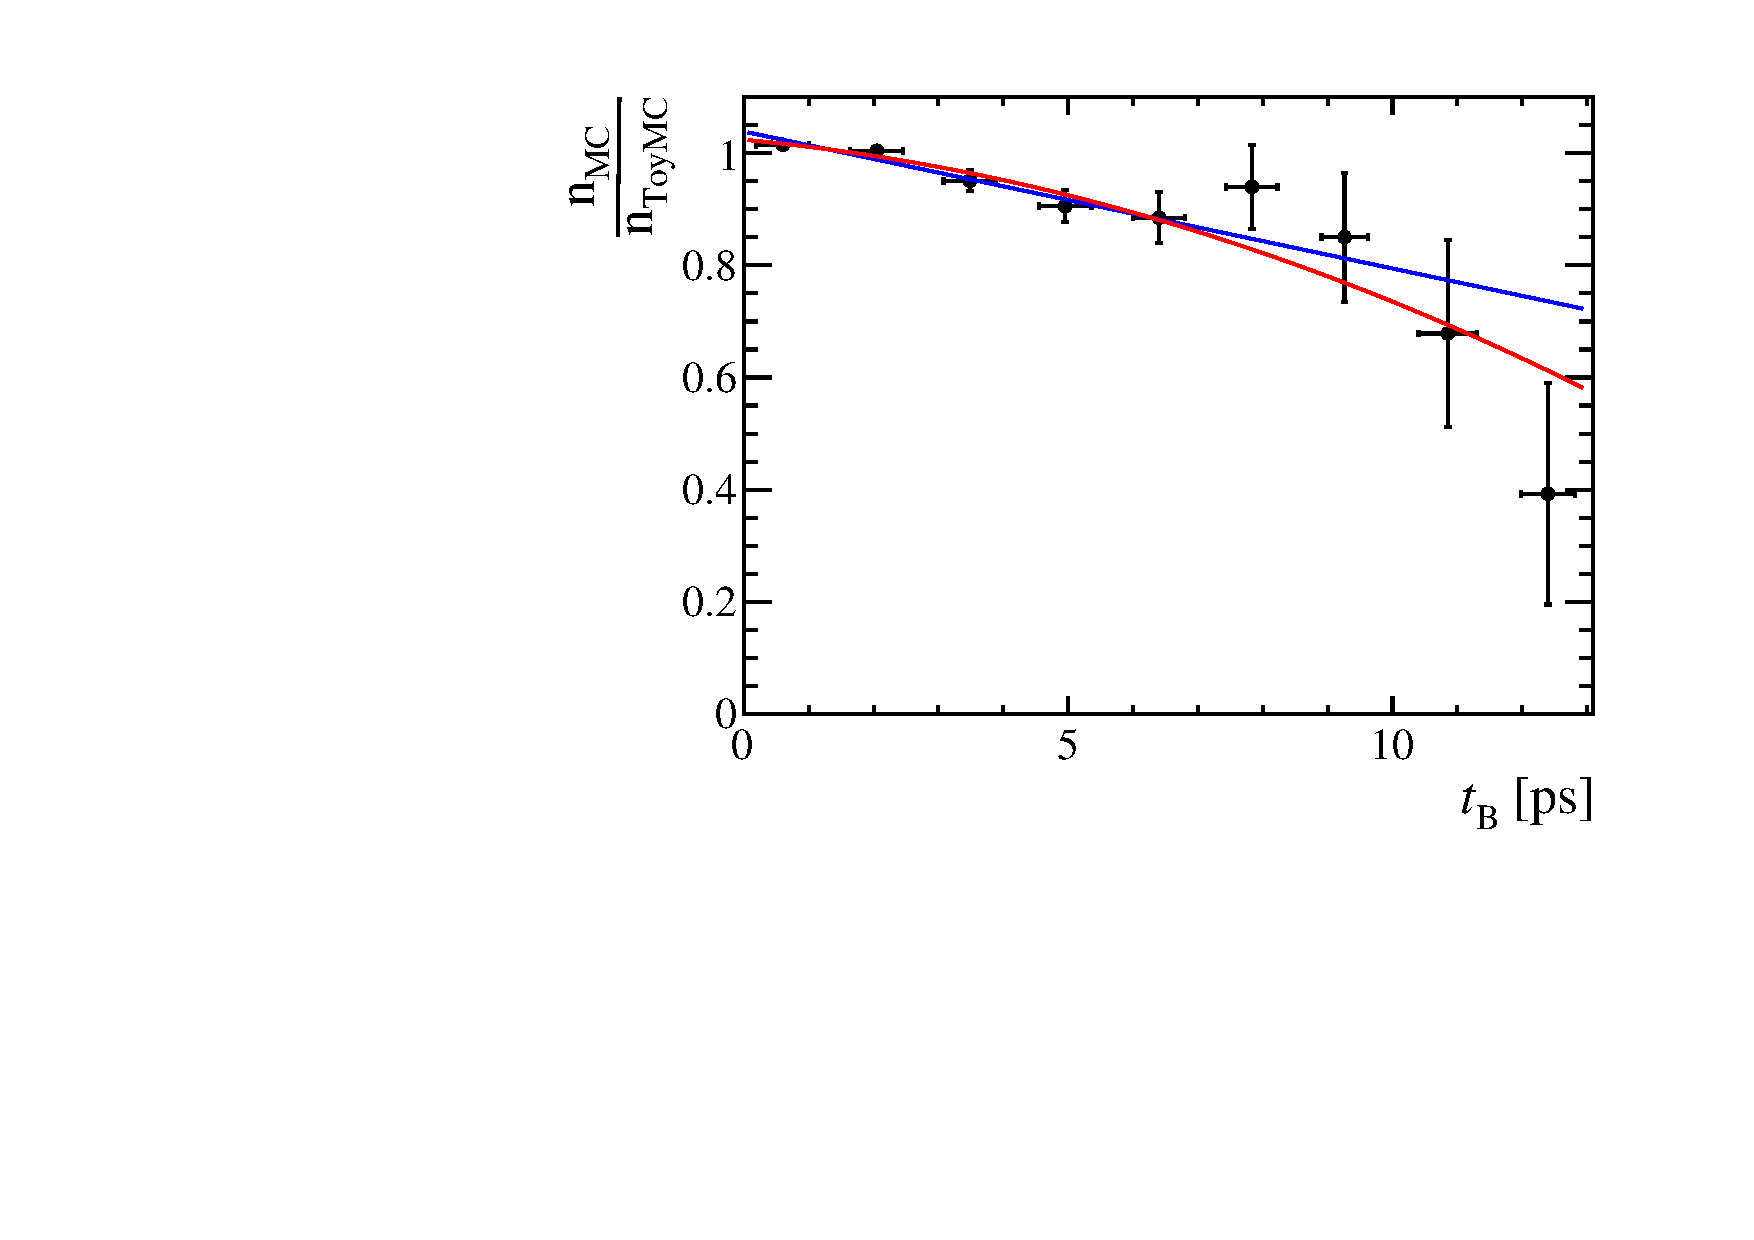
\includegraphics[width=0.49\textwidth]{private/content/measurement-of-sin2beta/figs/velo_acceptance_11_LL.pdf}
  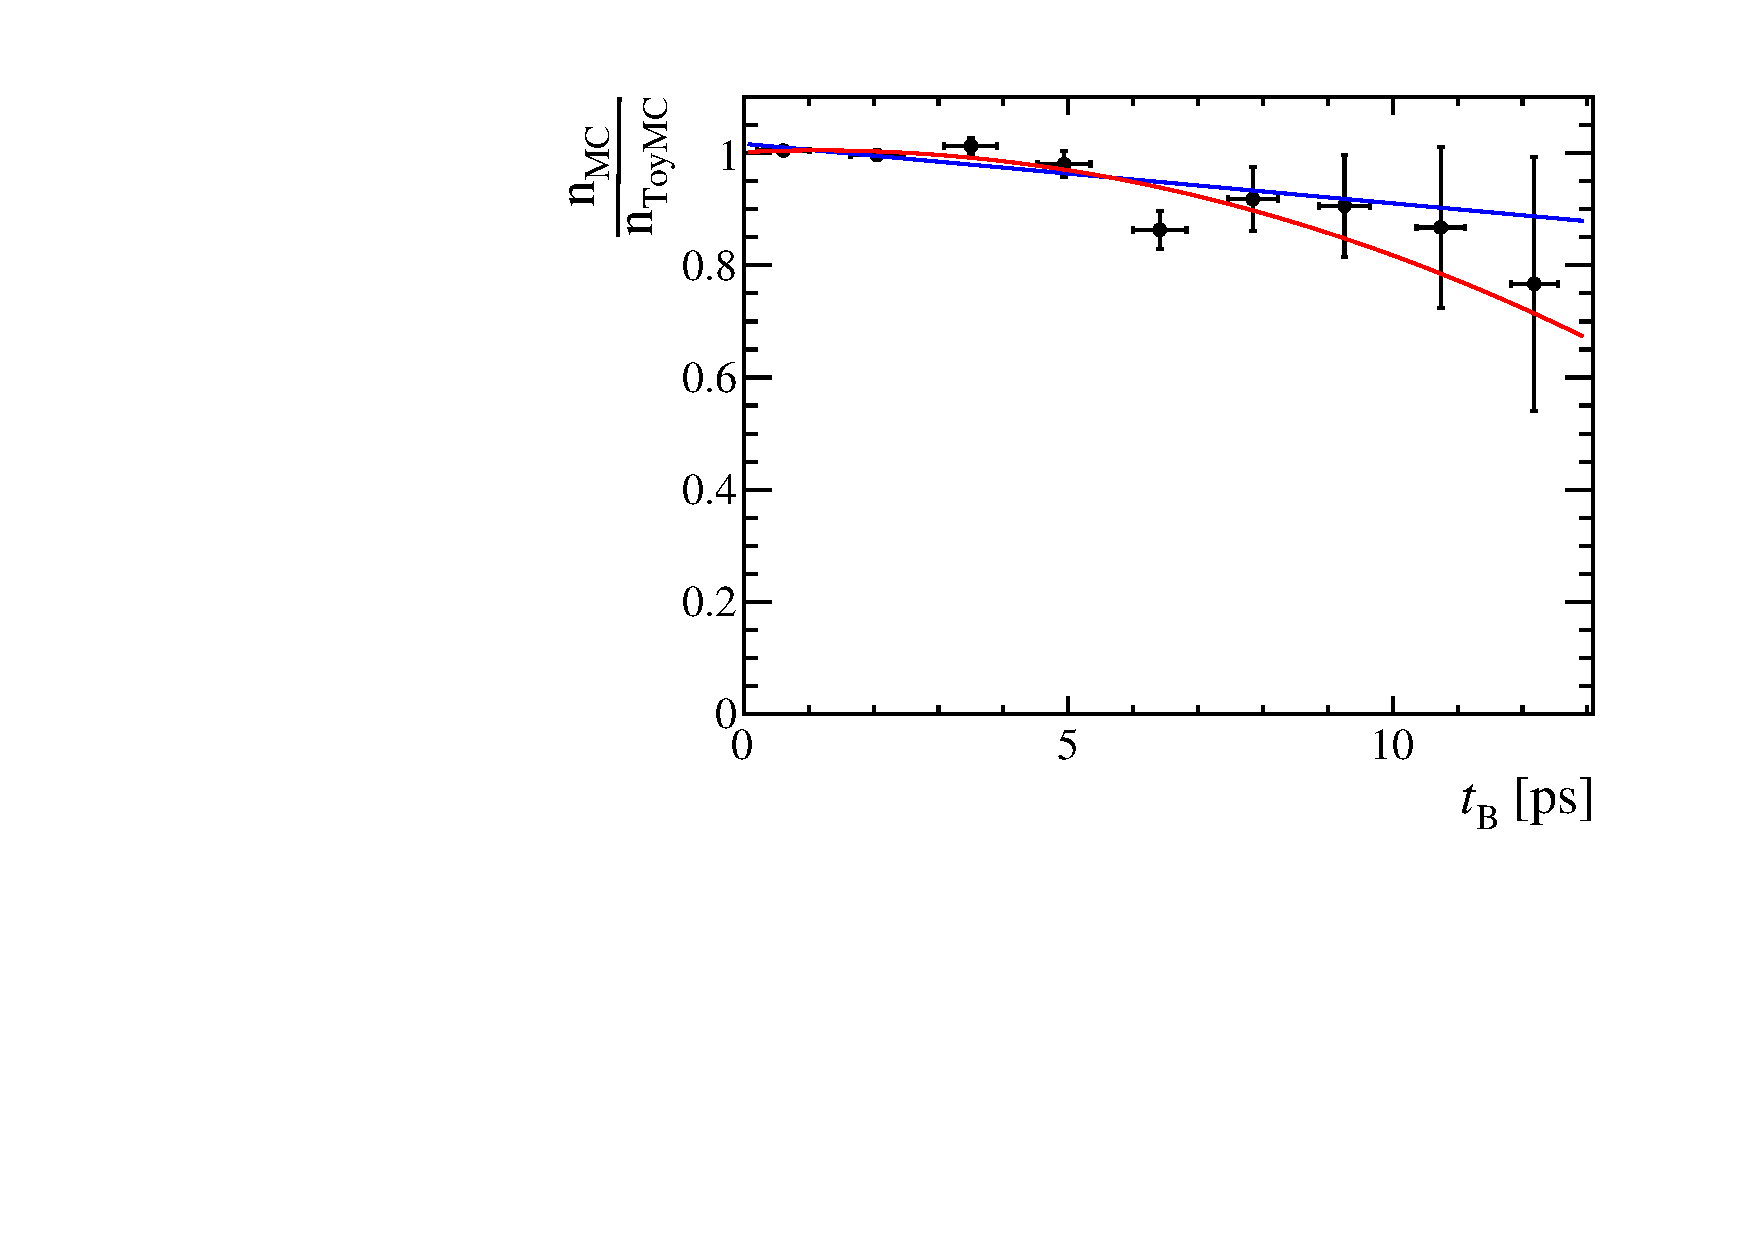
\includegraphics[width=0.49\textwidth]{private/content/measurement-of-sin2beta/figs/velo_acceptance_12_DD.pdf}\hfill
  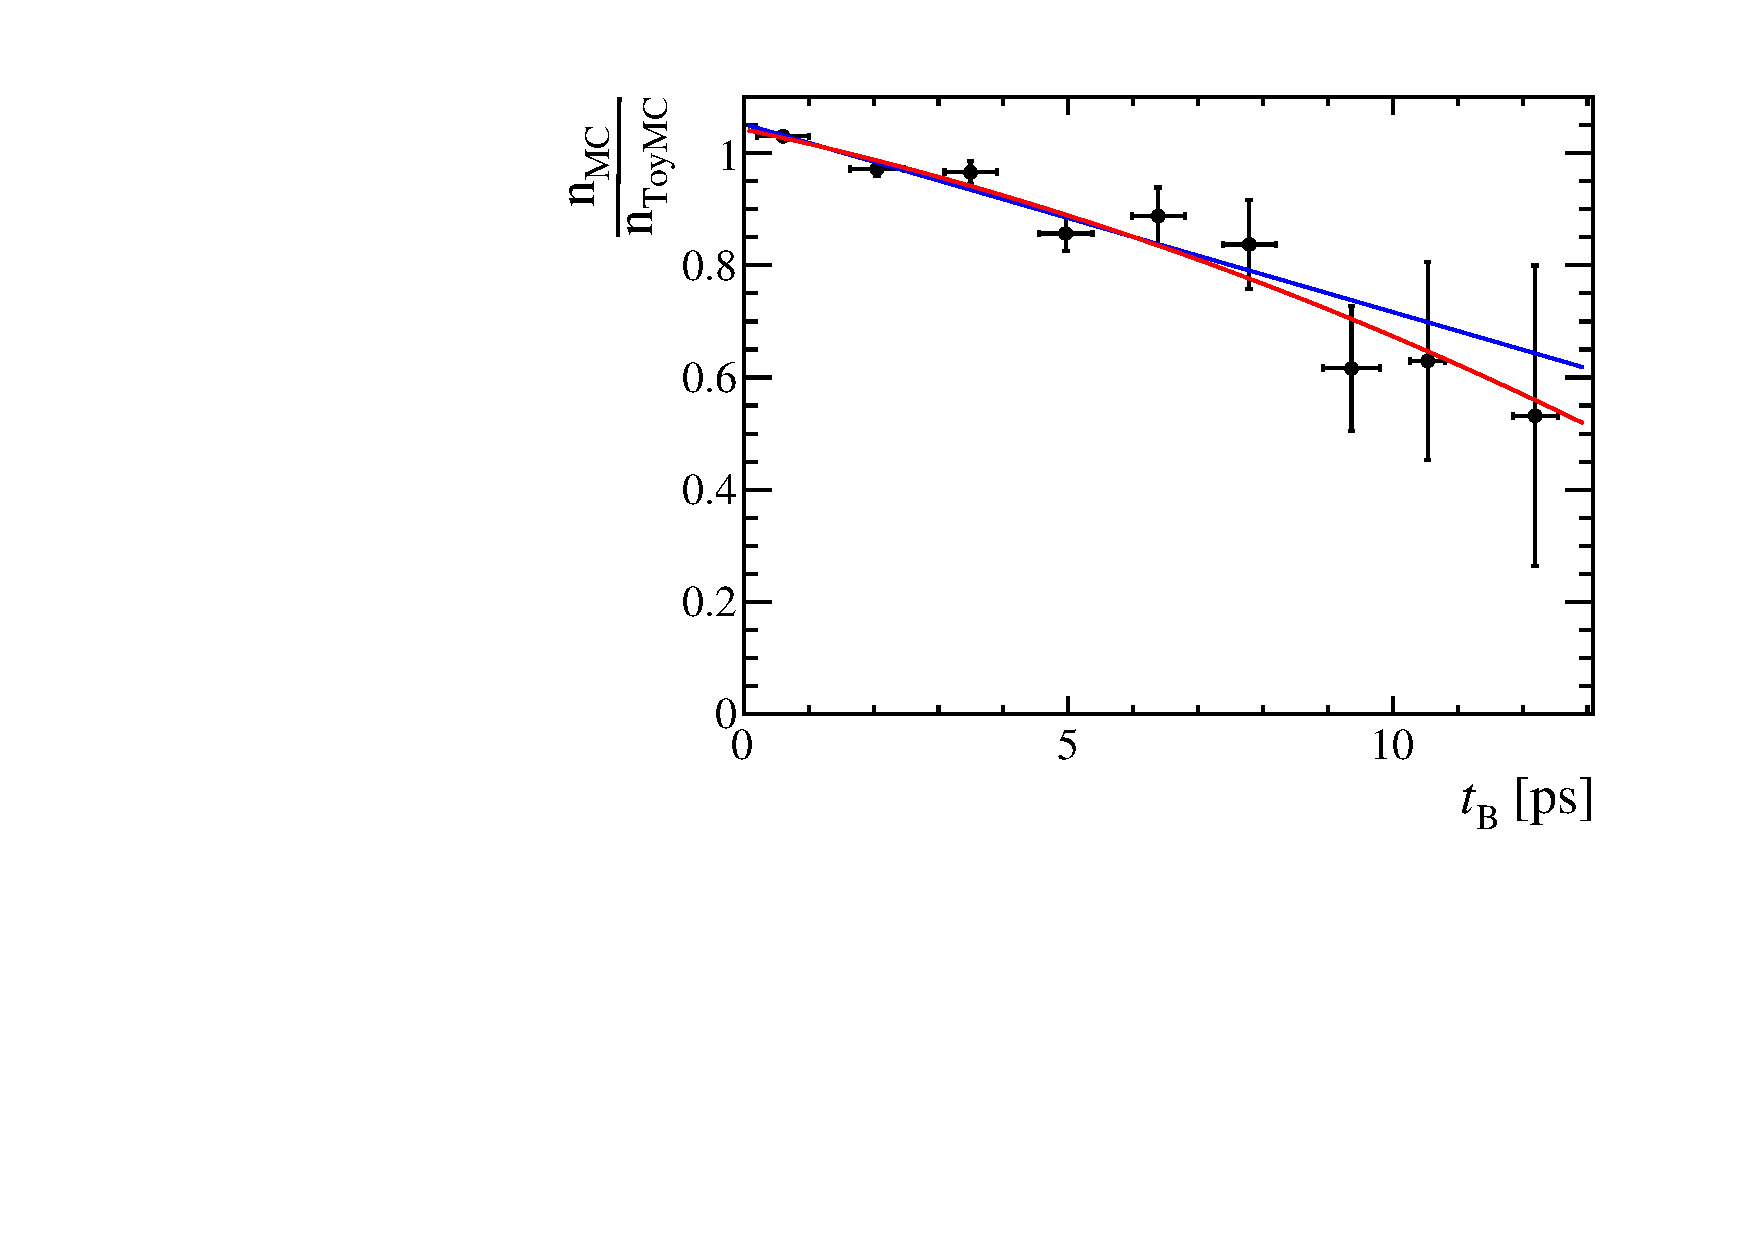
\includegraphics[width=0.49\textwidth]{private/content/measurement-of-sin2beta/figs/velo_acceptance_12_LL.pdf}
\caption{
Decay time ratio in bins of decay time for (left/right) \catDD/\catLL and
(top/bottom) \catOO/\catOT. The blue (red) curve shows a linear (quadratic) fit
to the data points.}
\label{fig:measurement_of_sin2beta:resolution_and_acceptance:acceptance:upper}
\end{figure}
